\documentclass[9pt]{article}

    \usepackage[breakable]{tcolorbox}
    \usepackage{parskip} % Stop auto-indenting (to mimic markdown behaviour)
    
    \usepackage{iftex}
    \ifPDFTeX
    	\usepackage[T1]{fontenc}
    	\usepackage{mathpazo}
    \else
    	\usepackage{fontspec}
    \fi

    % Basic figure setup, for now with no caption control since it's done
    % automatically by Pandoc (which extracts ![](path) syntax from Markdown).
    \usepackage{graphicx}
\usepackage[square,numbers]{natbib} 
\bibliographystyle{unsrtnat} 
    % Maintain compatibility with old templates. Remove in nbconvert 6.0
    \let\Oldincludegraphics\includegraphics
    % Ensure that by default, figures have no caption (until we provide a
    % proper Figure object with a Caption API and a way to capture that
    % in the conversion process - todo).
    \usepackage{caption}

    \usepackage{float}
    \floatplacement{figure}{H} % forces figures to be placed at the correct location
    \usepackage{xcolor} % Allow colors to be defined
    \usepackage{enumerate} % Needed for markdown enumerations to work
    \usepackage{geometry} % Used to adjust the document margins
    \usepackage{amsmath} % Equations
    \usepackage{amssymb} % Equations
    \usepackage{textcomp} % defines textquotesingle
    % Hack from http://tex.stackexchange.com/a/47451/13684:
    \AtBeginDocument{%
        \def\PYZsq{\textquotesingle}% Upright quotes in Pygmentized code
    }
    \usepackage{upquote} % Upright quotes for verbatim code
    \usepackage{eurosym} % defines \euro
    \usepackage[mathletters]{ucs} % Extended unicode (utf-8) support
    \usepackage{fancyvrb} % verbatim replacement that allows latex
    \usepackage{grffile} % extends the file name processing of package graphics 
                         % to support a larger range
    \makeatletter % fix for old versions of grffile with XeLaTeX
    \@ifpackagelater{grffile}{2019/11/01}
    {
      % Do nothing on new versions
    }
    {
      \def\Gread@@xetex#1{%
        \IfFileExists{"\Gin@base".bb}%
        {\Gread@eps{\Gin@base.bb}}%
        {\Gread@@xetex@aux#1}%
      }
    }
    \makeatother
    \usepackage[Export]{adjustbox} % Used to constrain images to a maximum size
    \adjustboxset{max size={0.9\linewidth}{0.9\paperheight}}

    % The hyperref package gives us a pdf with properly built
    % internal navigation ('pdf bookmarks' for the table of contents,
    % internal cross-reference links, web links for URLs, etc.)
    \usepackage{hyperref}
    % The default LaTeX title has an obnoxious amount of whitespace. By default,
    % titling removes some of it. It also provides customization options.
    \usepackage{titling}
    \usepackage{longtable} % longtable support required by pandoc >1.10
    \usepackage{booktabs}  % table support for pandoc > 1.12.2
    \usepackage[inline]{enumitem} % IRkernel/repr support (it uses the enumerate* environment)
    \usepackage[normalem]{ulem} % ulem is needed to support strikethroughs (\sout)
                                % normalem makes italics be italics, not underlines
    \usepackage{mathrsfs}
    

    
    % Colors for the hyperref package
    \definecolor{urlcolor}{rgb}{0,.145,.698}
    \definecolor{linkcolor}{rgb}{.71,0.21,0.01}
    \definecolor{citecolor}{rgb}{.12,.54,.11}

    % ANSI colors
    \definecolor{ansi-black}{HTML}{3E424D}
    \definecolor{ansi-black-intense}{HTML}{282C36}
    \definecolor{ansi-red}{HTML}{E75C58}
    \definecolor{ansi-red-intense}{HTML}{B22B31}
    \definecolor{ansi-green}{HTML}{00A250}
    \definecolor{ansi-green-intense}{HTML}{007427}
    \definecolor{ansi-yellow}{HTML}{DDB62B}
    \definecolor{ansi-yellow-intense}{HTML}{B27D12}
    \definecolor{ansi-blue}{HTML}{208FFB}
    \definecolor{ansi-blue-intense}{HTML}{0065CA}
    \definecolor{ansi-magenta}{HTML}{D160C4}
    \definecolor{ansi-magenta-intense}{HTML}{A03196}
    \definecolor{ansi-cyan}{HTML}{60C6C8}
    \definecolor{ansi-cyan-intense}{HTML}{258F8F}
    \definecolor{ansi-white}{HTML}{C5C1B4}
    \definecolor{ansi-white-intense}{HTML}{A1A6B2}
    \definecolor{ansi-default-inverse-fg}{HTML}{FFFFFF}
    \definecolor{ansi-default-inverse-bg}{HTML}{000000}

    % common color for the border for error outputs.
    \definecolor{outerrorbackground}{HTML}{FFDFDF}

    % commands and environments needed by pandoc snippets
    % extracted from the output of `pandoc -s`
    \providecommand{\tightlist}{%
      \setlength{\itemsep}{0pt}\setlength{\parskip}{0pt}}
    \DefineVerbatimEnvironment{Highlighting}{Verbatim}{commandchars=\\\{\}}
    % Add ',fontsize=\small' for more characters per line
    \newenvironment{Shaded}{}{}
    \newcommand{\KeywordTok}[1]{\textcolor[rgb]{0.00,0.44,0.13}{\textbf{{#1}}}}
    \newcommand{\DataTypeTok}[1]{\textcolor[rgb]{0.56,0.13,0.00}{{#1}}}
    \newcommand{\DecValTok}[1]{\textcolor[rgb]{0.25,0.63,0.44}{{#1}}}
    \newcommand{\BaseNTok}[1]{\textcolor[rgb]{0.25,0.63,0.44}{{#1}}}
    \newcommand{\FloatTok}[1]{\textcolor[rgb]{0.25,0.63,0.44}{{#1}}}
    \newcommand{\CharTok}[1]{\textcolor[rgb]{0.25,0.44,0.63}{{#1}}}
    \newcommand{\StringTok}[1]{\textcolor[rgb]{0.25,0.44,0.63}{{#1}}}
    \newcommand{\CommentTok}[1]{\textcolor[rgb]{0.38,0.63,0.69}{\textit{{#1}}}}
    \newcommand{\OtherTok}[1]{\textcolor[rgb]{0.00,0.44,0.13}{{#1}}}
    \newcommand{\AlertTok}[1]{\textcolor[rgb]{1.00,0.00,0.00}{\textbf{{#1}}}}
    \newcommand{\FunctionTok}[1]{\textcolor[rgb]{0.02,0.16,0.49}{{#1}}}
    \newcommand{\RegionMarkerTok}[1]{{#1}}
    \newcommand{\ErrorTok}[1]{\textcolor[rgb]{1.00,0.00,0.00}{\textbf{{#1}}}}
    \newcommand{\NormalTok}[1]{{#1}}
    
    % Additional commands for more recent versions of Pandoc
    \newcommand{\ConstantTok}[1]{\textcolor[rgb]{0.53,0.00,0.00}{{#1}}}
    \newcommand{\SpecialCharTok}[1]{\textcolor[rgb]{0.25,0.44,0.63}{{#1}}}
    \newcommand{\VerbatimStringTok}[1]{\textcolor[rgb]{0.25,0.44,0.63}{{#1}}}
    \newcommand{\SpecialStringTok}[1]{\textcolor[rgb]{0.73,0.40,0.53}{{#1}}}
    \newcommand{\ImportTok}[1]{{#1}}
    \newcommand{\DocumentationTok}[1]{\textcolor[rgb]{0.73,0.13,0.13}{\textit{{#1}}}}
    \newcommand{\AnnotationTok}[1]{\textcolor[rgb]{0.38,0.63,0.69}{\textbf{\textit{{#1}}}}}
    \newcommand{\CommentVarTok}[1]{\textcolor[rgb]{0.38,0.63,0.69}{\textbf{\textit{{#1}}}}}
    \newcommand{\VariableTok}[1]{\textcolor[rgb]{0.10,0.09,0.49}{{#1}}}
    \newcommand{\ControlFlowTok}[1]{\textcolor[rgb]{0.00,0.44,0.13}{\textbf{{#1}}}}
    \newcommand{\OperatorTok}[1]{\textcolor[rgb]{0.40,0.40,0.40}{{#1}}}
    \newcommand{\BuiltInTok}[1]{{#1}}
    \newcommand{\ExtensionTok}[1]{{#1}}
    \newcommand{\PreprocessorTok}[1]{\textcolor[rgb]{0.74,0.48,0.00}{{#1}}}
    \newcommand{\AttributeTok}[1]{\textcolor[rgb]{0.49,0.56,0.16}{{#1}}}
    \newcommand{\InformationTok}[1]{\textcolor[rgb]{0.38,0.63,0.69}{\textbf{\textit{{#1}}}}}
    \newcommand{\WarningTok}[1]{\textcolor[rgb]{0.38,0.63,0.69}{\textbf{\textit{{#1}}}}}
\newcommand{\onlinecite}[1]{\hspace{-1 ex} \nocite{#1}\citenum{#1}}    
    
    % Define a nice break command that doesn't care if a line doesn't already
    % exist.
    \def\br{\hspace*{\fill} \\* }
    % Math Jax compatibility definitions
    \def\gt{>}
    \def\lt{<}
    \let\Oldtex\TeX
    \let\Oldlatex\LaTeX
    \renewcommand{\TeX}{\textrm{\Oldtex}}
    \renewcommand{\LaTeX}{\textrm{\Oldlatex}}
    % Document parameters
    % Document title
\title{Accurate and efficient computation of mean ionization states with an average-atom Kubo--Greenwood approach: Supplementary Material} 
\author{Timothy J. Callow, Eli Kraisler, Attila Cangi}
    
    
    
    
    
% Pygments definitions
\makeatletter
\def\PY@reset{\let\PY@it=\relax \let\PY@bf=\relax%
    \let\PY@ul=\relax \let\PY@tc=\relax%
    \let\PY@bc=\relax \let\PY@ff=\relax}
\def\PY@tok#1{\csname PY@tok@#1\endcsname}
\def\PY@toks#1+{\ifx\relax#1\empty\else%
    \PY@tok{#1}\expandafter\PY@toks\fi}
\def\PY@do#1{\PY@bc{\PY@tc{\PY@ul{%
    \PY@it{\PY@bf{\PY@ff{#1}}}}}}}
\def\PY#1#2{\PY@reset\PY@toks#1+\relax+\PY@do{#2}}

\@namedef{PY@tok@w}{\def\PY@tc##1{\textcolor[rgb]{0.73,0.73,0.73}{##1}}}
\@namedef{PY@tok@c}{\let\PY@it=\textit\def\PY@tc##1{\textcolor[rgb]{0.25,0.50,0.50}{##1}}}
\@namedef{PY@tok@cp}{\def\PY@tc##1{\textcolor[rgb]{0.74,0.48,0.00}{##1}}}
\@namedef{PY@tok@k}{\let\PY@bf=\textbf\def\PY@tc##1{\textcolor[rgb]{0.00,0.50,0.00}{##1}}}
\@namedef{PY@tok@kp}{\def\PY@tc##1{\textcolor[rgb]{0.00,0.50,0.00}{##1}}}
\@namedef{PY@tok@kt}{\def\PY@tc##1{\textcolor[rgb]{0.69,0.00,0.25}{##1}}}
\@namedef{PY@tok@o}{\def\PY@tc##1{\textcolor[rgb]{0.40,0.40,0.40}{##1}}}
\@namedef{PY@tok@ow}{\let\PY@bf=\textbf\def\PY@tc##1{\textcolor[rgb]{0.67,0.13,1.00}{##1}}}
\@namedef{PY@tok@nb}{\def\PY@tc##1{\textcolor[rgb]{0.00,0.50,0.00}{##1}}}
\@namedef{PY@tok@nf}{\def\PY@tc##1{\textcolor[rgb]{0.00,0.00,1.00}{##1}}}
\@namedef{PY@tok@nc}{\let\PY@bf=\textbf\def\PY@tc##1{\textcolor[rgb]{0.00,0.00,1.00}{##1}}}
\@namedef{PY@tok@nn}{\let\PY@bf=\textbf\def\PY@tc##1{\textcolor[rgb]{0.00,0.00,1.00}{##1}}}
\@namedef{PY@tok@ne}{\let\PY@bf=\textbf\def\PY@tc##1{\textcolor[rgb]{0.82,0.25,0.23}{##1}}}
\@namedef{PY@tok@nv}{\def\PY@tc##1{\textcolor[rgb]{0.10,0.09,0.49}{##1}}}
\@namedef{PY@tok@no}{\def\PY@tc##1{\textcolor[rgb]{0.53,0.00,0.00}{##1}}}
\@namedef{PY@tok@nl}{\def\PY@tc##1{\textcolor[rgb]{0.63,0.63,0.00}{##1}}}
\@namedef{PY@tok@ni}{\let\PY@bf=\textbf\def\PY@tc##1{\textcolor[rgb]{0.60,0.60,0.60}{##1}}}
\@namedef{PY@tok@na}{\def\PY@tc##1{\textcolor[rgb]{0.49,0.56,0.16}{##1}}}
\@namedef{PY@tok@nt}{\let\PY@bf=\textbf\def\PY@tc##1{\textcolor[rgb]{0.00,0.50,0.00}{##1}}}
\@namedef{PY@tok@nd}{\def\PY@tc##1{\textcolor[rgb]{0.67,0.13,1.00}{##1}}}
\@namedef{PY@tok@s}{\def\PY@tc##1{\textcolor[rgb]{0.73,0.13,0.13}{##1}}}
\@namedef{PY@tok@sd}{\let\PY@it=\textit\def\PY@tc##1{\textcolor[rgb]{0.73,0.13,0.13}{##1}}}
\@namedef{PY@tok@si}{\let\PY@bf=\textbf\def\PY@tc##1{\textcolor[rgb]{0.73,0.40,0.53}{##1}}}
\@namedef{PY@tok@se}{\let\PY@bf=\textbf\def\PY@tc##1{\textcolor[rgb]{0.73,0.40,0.13}{##1}}}
\@namedef{PY@tok@sr}{\def\PY@tc##1{\textcolor[rgb]{0.73,0.40,0.53}{##1}}}
\@namedef{PY@tok@ss}{\def\PY@tc##1{\textcolor[rgb]{0.10,0.09,0.49}{##1}}}
\@namedef{PY@tok@sx}{\def\PY@tc##1{\textcolor[rgb]{0.00,0.50,0.00}{##1}}}
\@namedef{PY@tok@m}{\def\PY@tc##1{\textcolor[rgb]{0.40,0.40,0.40}{##1}}}
\@namedef{PY@tok@gh}{\let\PY@bf=\textbf\def\PY@tc##1{\textcolor[rgb]{0.00,0.00,0.50}{##1}}}
\@namedef{PY@tok@gu}{\let\PY@bf=\textbf\def\PY@tc##1{\textcolor[rgb]{0.50,0.00,0.50}{##1}}}
\@namedef{PY@tok@gd}{\def\PY@tc##1{\textcolor[rgb]{0.63,0.00,0.00}{##1}}}
\@namedef{PY@tok@gi}{\def\PY@tc##1{\textcolor[rgb]{0.00,0.63,0.00}{##1}}}
\@namedef{PY@tok@gr}{\def\PY@tc##1{\textcolor[rgb]{1.00,0.00,0.00}{##1}}}
\@namedef{PY@tok@ge}{\let\PY@it=\textit}
\@namedef{PY@tok@gs}{\let\PY@bf=\textbf}
\@namedef{PY@tok@gp}{\let\PY@bf=\textbf\def\PY@tc##1{\textcolor[rgb]{0.00,0.00,0.50}{##1}}}
\@namedef{PY@tok@go}{\def\PY@tc##1{\textcolor[rgb]{0.53,0.53,0.53}{##1}}}
\@namedef{PY@tok@gt}{\def\PY@tc##1{\textcolor[rgb]{0.00,0.27,0.87}{##1}}}
\@namedef{PY@tok@err}{\def\PY@bc##1{{\setlength{\fboxsep}{\string -\fboxrule}\fcolorbox[rgb]{1.00,0.00,0.00}{1,1,1}{\strut ##1}}}}
\@namedef{PY@tok@kc}{\let\PY@bf=\textbf\def\PY@tc##1{\textcolor[rgb]{0.00,0.50,0.00}{##1}}}
\@namedef{PY@tok@kd}{\let\PY@bf=\textbf\def\PY@tc##1{\textcolor[rgb]{0.00,0.50,0.00}{##1}}}
\@namedef{PY@tok@kn}{\let\PY@bf=\textbf\def\PY@tc##1{\textcolor[rgb]{0.00,0.50,0.00}{##1}}}
\@namedef{PY@tok@kr}{\let\PY@bf=\textbf\def\PY@tc##1{\textcolor[rgb]{0.00,0.50,0.00}{##1}}}
\@namedef{PY@tok@bp}{\def\PY@tc##1{\textcolor[rgb]{0.00,0.50,0.00}{##1}}}
\@namedef{PY@tok@fm}{\def\PY@tc##1{\textcolor[rgb]{0.00,0.00,1.00}{##1}}}
\@namedef{PY@tok@vc}{\def\PY@tc##1{\textcolor[rgb]{0.10,0.09,0.49}{##1}}}
\@namedef{PY@tok@vg}{\def\PY@tc##1{\textcolor[rgb]{0.10,0.09,0.49}{##1}}}
\@namedef{PY@tok@vi}{\def\PY@tc##1{\textcolor[rgb]{0.10,0.09,0.49}{##1}}}
\@namedef{PY@tok@vm}{\def\PY@tc##1{\textcolor[rgb]{0.10,0.09,0.49}{##1}}}
\@namedef{PY@tok@sa}{\def\PY@tc##1{\textcolor[rgb]{0.73,0.13,0.13}{##1}}}
\@namedef{PY@tok@sb}{\def\PY@tc##1{\textcolor[rgb]{0.73,0.13,0.13}{##1}}}
\@namedef{PY@tok@sc}{\def\PY@tc##1{\textcolor[rgb]{0.73,0.13,0.13}{##1}}}
\@namedef{PY@tok@dl}{\def\PY@tc##1{\textcolor[rgb]{0.73,0.13,0.13}{##1}}}
\@namedef{PY@tok@s2}{\def\PY@tc##1{\textcolor[rgb]{0.73,0.13,0.13}{##1}}}
\@namedef{PY@tok@sh}{\def\PY@tc##1{\textcolor[rgb]{0.73,0.13,0.13}{##1}}}
\@namedef{PY@tok@s1}{\def\PY@tc##1{\textcolor[rgb]{0.73,0.13,0.13}{##1}}}
\@namedef{PY@tok@mb}{\def\PY@tc##1{\textcolor[rgb]{0.40,0.40,0.40}{##1}}}
\@namedef{PY@tok@mf}{\def\PY@tc##1{\textcolor[rgb]{0.40,0.40,0.40}{##1}}}
\@namedef{PY@tok@mh}{\def\PY@tc##1{\textcolor[rgb]{0.40,0.40,0.40}{##1}}}
\@namedef{PY@tok@mi}{\def\PY@tc##1{\textcolor[rgb]{0.40,0.40,0.40}{##1}}}
\@namedef{PY@tok@il}{\def\PY@tc##1{\textcolor[rgb]{0.40,0.40,0.40}{##1}}}
\@namedef{PY@tok@mo}{\def\PY@tc##1{\textcolor[rgb]{0.40,0.40,0.40}{##1}}}
\@namedef{PY@tok@ch}{\let\PY@it=\textit\def\PY@tc##1{\textcolor[rgb]{0.25,0.50,0.50}{##1}}}
\@namedef{PY@tok@cm}{\let\PY@it=\textit\def\PY@tc##1{\textcolor[rgb]{0.25,0.50,0.50}{##1}}}
\@namedef{PY@tok@cpf}{\let\PY@it=\textit\def\PY@tc##1{\textcolor[rgb]{0.25,0.50,0.50}{##1}}}
\@namedef{PY@tok@c1}{\let\PY@it=\textit\def\PY@tc##1{\textcolor[rgb]{0.25,0.50,0.50}{##1}}}
\@namedef{PY@tok@cs}{\let\PY@it=\textit\def\PY@tc##1{\textcolor[rgb]{0.25,0.50,0.50}{##1}}}

\def\PYZbs{\char`\\}
\def\PYZus{\char`\_}
\def\PYZob{\char`\{}
\def\PYZcb{\char`\}}
\def\PYZca{\char`\^}
\def\PYZam{\char`\&}
\def\PYZlt{\char`\<}
\def\PYZgt{\char`\>}
\def\PYZsh{\char`\#}
\def\PYZpc{\char`\%}
\def\PYZdl{\char`\$}
\def\PYZhy{\char`\-}
\def\PYZsq{\char`\'}
\def\PYZdq{\char`\"}
\def\PYZti{\char`\~}
% for compatibility with earlier versions
\def\PYZat{@}
\def\PYZlb{[}
\def\PYZrb{]}
\makeatother


    % For linebreaks inside Verbatim environment from package fancyvrb. 
    \makeatletter
        \newbox\Wrappedcontinuationbox 
        \newbox\Wrappedvisiblespacebox 
        \newcommand*\Wrappedvisiblespace {\textcolor{red}{\textvisiblespace}} 
        \newcommand*\Wrappedcontinuationsymbol {\textcolor{red}{\llap{\tiny$\m@th\hookrightarrow$}}} 
        \newcommand*\Wrappedcontinuationindent {3ex } 
        \newcommand*\Wrappedafterbreak {\kern\Wrappedcontinuationindent\copy\Wrappedcontinuationbox} 
        % Take advantage of the already applied Pygments mark-up to insert 
        % potential linebreaks for TeX processing. 
        %        {, <, #, %, $, ' and ": go to next line. 
        %        _, }, ^, &, >, - and ~: stay at end of broken line. 
        % Use of \textquotesingle for straight quote. 
        \newcommand*\Wrappedbreaksatspecials {% 
            \def\PYGZus{\discretionary{\char`\_}{\Wrappedafterbreak}{\char`\_}}% 
            \def\PYGZob{\discretionary{}{\Wrappedafterbreak\char`\{}{\char`\{}}% 
            \def\PYGZcb{\discretionary{\char`\}}{\Wrappedafterbreak}{\char`\}}}% 
            \def\PYGZca{\discretionary{\char`\^}{\Wrappedafterbreak}{\char`\^}}% 
            \def\PYGZam{\discretionary{\char`\&}{\Wrappedafterbreak}{\char`\&}}% 
            \def\PYGZlt{\discretionary{}{\Wrappedafterbreak\char`\<}{\char`\<}}% 
            \def\PYGZgt{\discretionary{\char`\>}{\Wrappedafterbreak}{\char`\>}}% 
            \def\PYGZsh{\discretionary{}{\Wrappedafterbreak\char`\#}{\char`\#}}% 
            \def\PYGZpc{\discretionary{}{\Wrappedafterbreak\char`\%}{\char`\%}}% 
            \def\PYGZdl{\discretionary{}{\Wrappedafterbreak\char`\$}{\char`\$}}% 
            \def\PYGZhy{\discretionary{\char`\-}{\Wrappedafterbreak}{\char`\-}}% 
            \def\PYGZsq{\discretionary{}{\Wrappedafterbreak\textquotesingle}{\textquotesingle}}% 
            \def\PYGZdq{\discretionary{}{\Wrappedafterbreak\char`\"}{\char`\"}}% 
            \def\PYGZti{\discretionary{\char`\~}{\Wrappedafterbreak}{\char`\~}}% 
        } 
        % Some characters . , ; ? ! / are not pygmentized. 
        % This macro makes them "active" and they will insert potential linebreaks 
        \newcommand*\Wrappedbreaksatpunct {% 
            \lccode`\~`\.\lowercase{\def~}{\discretionary{\hbox{\char`\.}}{\Wrappedafterbreak}{\hbox{\char`\.}}}% 
            \lccode`\~`\,\lowercase{\def~}{\discretionary{\hbox{\char`\,}}{\Wrappedafterbreak}{\hbox{\char`\,}}}% 
            \lccode`\~`\;\lowercase{\def~}{\discretionary{\hbox{\char`\;}}{\Wrappedafterbreak}{\hbox{\char`\;}}}% 
            \lccode`\~`\:\lowercase{\def~}{\discretionary{\hbox{\char`\:}}{\Wrappedafterbreak}{\hbox{\char`\:}}}% 
            \lccode`\~`\?\lowercase{\def~}{\discretionary{\hbox{\char`\?}}{\Wrappedafterbreak}{\hbox{\char`\?}}}% 
            \lccode`\~`\!\lowercase{\def~}{\discretionary{\hbox{\char`\!}}{\Wrappedafterbreak}{\hbox{\char`\!}}}% 
            \lccode`\~`\/\lowercase{\def~}{\discretionary{\hbox{\char`\/}}{\Wrappedafterbreak}{\hbox{\char`\/}}}% 
            \catcode`\.\active
            \catcode`\,\active 
            \catcode`\;\active
            \catcode`\:\active
            \catcode`\?\active
            \catcode`\!\active
            \catcode`\/\active 
            \lccode`\~`\~ 	
        }
    \makeatother

    \let\OriginalVerbatim=\Verbatim
    \makeatletter
    \renewcommand{\Verbatim}[1][1]{%
        %\parskip\z@skip
        \sbox\Wrappedcontinuationbox {\Wrappedcontinuationsymbol}%
        \sbox\Wrappedvisiblespacebox {\FV@SetupFont\Wrappedvisiblespace}%
        \def\FancyVerbFormatLine ##1{\hsize\linewidth
            \vtop{\raggedright\hyphenpenalty\z@\exhyphenpenalty\z@
                \doublehyphendemerits\z@\finalhyphendemerits\z@
                \strut ##1\strut}%
        }%
        % If the linebreak is at a space, the latter will be displayed as visible
        % space at end of first line, and a continuation symbol starts next line.
        % Stretch/shrink are however usually zero for typewriter font.
        \def\FV@Space {%
            \nobreak\hskip\z@ plus\fontdimen3\font minus\fontdimen4\font
            \discretionary{\copy\Wrappedvisiblespacebox}{\Wrappedafterbreak}
            {\kern\fontdimen2\font}%
        }%
        
        % Allow breaks at special characters using \PYG... macros.
        \Wrappedbreaksatspecials
        % Breaks at punctuation characters . , ; ? ! and / need catcode=\active 	
        \OriginalVerbatim[#1,codes*=\Wrappedbreaksatpunct]%
    }
    \makeatother

    % Exact colors from NB
    \definecolor{incolor}{HTML}{303F9F}
    \definecolor{outcolor}{HTML}{D84315}
    \definecolor{cellborder}{HTML}{CFCFCF}
    \definecolor{cellbackground}{HTML}{F7F7F7}
    
    % prompt
    \makeatletter
    \newcommand{\boxspacing}{\kern\kvtcb@left@rule\kern\kvtcb@boxsep}
    \makeatother
    \newcommand{\prompt}[4]{
        {\ttfamily\llap{{\color{#2}[#3]:\hspace{3pt}#4}}\vspace{-\baselineskip}}
    }
    

    
    % Prevent overflowing lines due to hard-to-break entities
    \sloppy 
    % Setup hyperref package
    \hypersetup{
      breaklinks=true,  % so long urls are correctly broken across lines
      colorlinks=true,
      urlcolor=urlcolor,
      linkcolor=linkcolor,
      citecolor=citecolor,
      }
    % Slightly bigger margins than the latex defaults
    
    \geometry{verbose,tmargin=1in,bmargin=1in,lmargin=1in,rmargin=1in}
    
    

\begin{document}
    
    \maketitle
    
    

    
    \hypertarget{average-atom-models-theoretical-background}{%
\section{Average atom models: Theoretical
background}\label{average-atom-models-theoretical-background}}

In this section, we describe the average-atom model that we use and the
equations that are solved. For a detailed derivation and discussion of
the model, please see our earlier pre-print
\cite{callow2021firstprinciples}. As noted in the main text, the most
important difference from this previous model is that we do not now
distinguish between bound and free KS orbitals, but rather all orbitals
follow from the same KS equations and boundary conditions. The second
difference is that, in this paper, we solve the spin-unpolarized KS
equations; in other words, the spatial spin-up and spin-down orbitals
are assumed to be identical,
\(\phi_i^\uparrow(\vec{r})=\phi_i^\downarrow(\vec{r})\).

We shall first review the important aspects of our model; in the
following sub-section, we explain in more detail the band-structure
model of Massacrier \emph{et al.} \cite{massacrier_bands} which we have
also implemented in atoMEC. As discussed in the main text, we solve the
spherically symmetric Kohn--Sham (KS) equations for an atom at finite
temperature, with appropriate boundary conditions imposed on the
orbitals intended to mimic the effect of interactions from electrons and
nuclei in neighbouring atoms. The spherically symmetric KS equations are
given by

\begin{equation}
\left[\frac{\textrm{d}^2}{\textrm{d}r} + \frac{2}{r}\frac{\textrm{d}}{\textrm{d}r} - \frac{l(l+1)}{r^2} \right] X_{nl}(r) + 2 \left[\epsilon^{\tau}_{nl} - v_\textrm{s}[n](r) \right] X_{nl}(r) = 0,
\end{equation}

where \(v_\textrm{s}[n](r)\) is the KS potential, given by

\begin{equation}
 v_{\textrm{s}}[n](r) = -\frac{Z}{r} + 4\pi \int_0^{R_\textrm{WS}} \textrm{d}{x} \frac{n(x)x^2}{r^>(x)} + \frac{\delta F_\textrm{xc}^\tau [n]}{\delta n(r)}\,,
\end{equation}

where \(r^>(x)=\max(r,x)\). The three terms in the potential are
respectively the electron-nuclear attraction, the classical Hartree
repulsion, and the exchange-correlation (xc) potential, which is equal
to the functional derivative of the xc free energy. As ever, due to the
dependence of the KS potential on the density \(n(r)\), the KS equations
must be solved iteratively until self-consistency is reached.

The density \(n(r)\) is constructed from the orbitals as

\begin{equation}
n(r) = 2\sum_{nl}(2l+1) f_{nl}(\epsilon_{nl},\mu,\tau) |X_{nl}(r)|^2\,.
\end{equation}

where \(f_{nl}(\epsilon_{nl},\mu,\tau)\) the Fermi--Dirac (FD)
distribution, given by

\begin{equation}
f_{nl}(\epsilon_{nl},\mu,\tau) = \frac{1}{1+e^{(\epsilon_{nl}-\mu)/\tau}}\,.
\end{equation}

The chemical potential \(\mu\) is determined by fixing the electron
number \(N_\textrm{e}=4\pi\int\textrm{d}r r^2 n(r)\) to be equal to a
pre-determined value (in this paper, \(N_\textrm{e}=Z\) in all cases).

As discussed in the main text, we impose boundary conditions on the KS
orbitals \(X_{nl}(r)\) which are intended to implicitly account for
inter-atomic interactions. In our earlier preprint
\cite{callow2021firstprinciples}, we argued that a physically intuitive
condition was to impose smoothness of the density at the edge of the WS
cell,

\begin{equation}
\frac{\textrm{d}n(r)}{\textrm{d}r}\Bigg|_{r=R_\textrm{WS}} =0\,.
\end{equation}

Mathematically there is no unique way to enforce the above condition,
but two simple choices are

\begin{align}
0&=X_{nl}(R_\textrm{VS})\,, \\
0&=\frac{\textrm{d}X_{nl}(r)}{\textrm{d}r}\Bigg|_{r=R_\textrm{WS}}\,,
\end{align}

which we refer to respectively as ``Dirichlet'' and ``Neumann''
conditions. As discussed in the main text, the energy eigenvalues that
result from these boundary conditions also define the upper and lower
energy band limits \(\epsilon^{\pm}_{nl}\) for the band-structure model.
We elaborate on this model in the following sub-section.

\hypertarget{band-structure-aa-model}{%
\subsection{Band-structure AA model}\label{band-structure-aa-model}}

We here elaborate on the band-structure model proposed by Massacrier
\emph{et al}, which we have implemented in atoMEC. In this model, the
orbitals gain an extra index since we solve the KS equations for all
energies in a given band. The KS equations thus become

\begin{equation}
\left[\frac{\textrm{d}^2}{\textrm{d}r} + \frac{2}{r}\frac{\textrm{d}}{\textrm{d}r} - \frac{l(l+1)}{r^2} \right] X_{\epsilon nl}(r) + 2 \left[\epsilon^{\tau}_{nl} - v_\textrm{s}[n](r) \right] X_{\epsilon nl}(r) = 0,
\end{equation}

and the density is given by

\begin{equation}
    n(r) = 2\sum_{nl}(2l+1)
    \int_{\epsilon_{nl}^-}^{\epsilon_{nl}^+} \textrm{d}{\epsilon} g_{nl}(\epsilon) f_{nl}(\epsilon,\mu,\tau) |X_{nl\epsilon}(r)|^2\,,
\end{equation}

with the density-of-states (DOS) \(g_{nl}(\epsilon)\) given by the
Hubbard DOS,

\begin{gather}
g_{nl}(\epsilon) =\frac{8}{ \pi \Delta_{nl}^2} \sqrt{(\epsilon^+_{nl}-\epsilon)(\epsilon - \epsilon^-_{nl})}\,,\\
\Delta_{nl} = \epsilon^+_{nl}-\epsilon_{nl}^- \,.
\end{gather}

In practise, the energy bands are of discretized, and the above integral
becomes a summation over energies within each band which we now denote
by index \(k\),

\begin{gather}
 n(r) = 2\sum_{knl}(2l+1) \delta\epsilon_{knl} g_{knl}(\epsilon_{knl},\epsilon_{nl}^\pm) f_{knl}(\epsilon_{knl},\mu,\tau) |X_{knl}(r)|^2\,,\\
 g_{knl}(\epsilon_{knl},\epsilon_{nl}^\pm) =\frac{8}{ \pi \Delta_{nl}^2} \sqrt{(\epsilon^+_{nl}-\epsilon_{knl})(\epsilon_{knl} - \epsilon^-_{nl})}\,.
\end{gather}

We now simplify the above expressions. To the best of our knowledge,
this simplification was not discussed in the original paper. Firstly, we
note that the energy spacing in the discretization of the energy band
\(\delta\epsilon_{knl}\) can be written as

\begin{equation}
\delta\epsilon_{knl} = \frac{\epsilon^+_{nl} - \epsilon^-_{nl}}{N_k-1} = \frac{\Delta_{nl}}{N_k-1}\,,
\end{equation}

where \(N_k\) is the number of \(k\) points (the denominator is equal to
\(N_k-1\) because there are \(N_k-1\) spacings for \(N_k\) total
points). The product
\(\delta\epsilon_{knl} \times g_{knl}(\epsilon_{knl},\epsilon_{nl}^\pm)\)
therefore can be written as

\begin{equation}
\delta\epsilon_{knl} \times g_{knl}(\epsilon_{knl},\epsilon_{nl}^\pm) = \frac{8}{\pi\Delta_{nl}(N_k-1)} \sqrt{(\epsilon^+_{nl}-\epsilon_{knl})(\epsilon_{knl} - \epsilon^-_{nl})}\,.
\end{equation}

We then note that the energies in a band \(\epsilon_{knl}\) can be
re-written as \begin{align}
\epsilon_{knl} &= \epsilon_{nl}^- + \frac{k}{N_k-1}\Delta_{nl} \\
               &= \epsilon_{nl}^+ + \frac{k-(N_k-1)}{N_k-1}\Delta_{nl}
\end{align}

Substituting the above expressions into the product
\(\delta\epsilon_{knl} \times g_{knl}(\epsilon_{knl},\epsilon_{nl}^\pm)\)
leads to the following expression:

\begin{equation}
\delta\epsilon_{knl} \times g_{knl}(\epsilon_{knl},\epsilon_{nl}^\pm) = \frac{8}{\pi(N_k-1)^2}\sqrt{k(N_k-1-k)}\,.
\end{equation}

It is clear the above equation is in fact independent of the quantum
numbers \(n\) and \(l\). The density \(n(r)\) can therefore be
re-expressed as

\begin{gather}
n(r) = 2\sum_{k} w_k \sum_{nl}(2l+1) f_{knl}(\epsilon_{knl},\mu,\tau) |X_{knl}(r)|^2\,,\\
w_k = \frac{8}{\pi(N_k-1)^2}\sqrt{k(N_k-1-k)} \Rightarrow \sum_{k=0}^{N_k-1} w_k =1\,.
\end{gather}

The above expression closely resembles the expression for the density in
plane-wave DFT codes, since it has a summation over \(k\)-points and
some weighting \(w_k\), very much like the \(\vec{k}\) point mesh for
reciporacal space used in plane-wave DFT codes. It is also clear to see
that when the concept of bands in the AA model is not employed
(i.e.~when we use either the Dirichlet or Neumann conditions only), that
\(N_k=1,w_k=1\) and the above expression reduces to the expression for
the density in the previous sub-section.

    \hypertarget{introduction-to-atomec}{%
\section{Introduction to atoMEC}\label{introduction-to-atomec}}

For all calculations in the paper, we have used the open source
average-atom code atoMEC. It can be downloaded from Ref.
\onlinecite{atoMEC}.

In this section, we go through the basics of setting up and then running
a calcuation in atoMEC.

We first create an \texttt{Atom} object which houses the key physical
information about the system we want to study, i.e.~the temperature and
mass density. We start with Aluminium at room temperature:

    \begin{tcolorbox}[breakable, size=fbox, boxrule=1pt, pad at break*=1mm,colback=cellbackground, colframe=cellborder]
\prompt{In}{incolor}{1}{\boxspacing}
\begin{Verbatim}[commandchars=\\\{\}]
\PY{c+c1}{\PYZsh{} first: general set\PYZhy{}up and imports}
\PY{o}{\PYZpc{}}\PY{k}{load\PYZus{}ext} autoreload
\PY{o}{\PYZpc{}}\PY{k}{autoreload} 2

\PY{k+kn}{import} \PY{n+nn}{sys}
\PY{k+kn}{import} \PY{n+nn}{os}
\PY{k+kn}{import} \PY{n+nn}{matplotlib}\PY{n+nn}{.}\PY{n+nn}{pyplot} \PY{k}{as} \PY{n+nn}{plt}
\PY{k+kn}{import} \PY{n+nn}{numpy} \PY{k}{as} \PY{n+nn}{np}
\PY{k+kn}{import} \PY{n+nn}{MIS\PYZus{}plots}

\PY{c+c1}{\PYZsh{} set the default printing output}
\PY{n}{default\PYZus{}stdout} \PY{o}{=} \PY{n}{sys}\PY{o}{.}\PY{n}{stdout}
\PY{c+c1}{\PYZsh{} base directory:}
\PY{n}{basedir} \PY{o}{=} \PY{n}{os}\PY{o}{.}\PY{n}{getcwd}\PY{p}{(}\PY{p}{)}
\end{Verbatim}
\end{tcolorbox}

    \begin{tcolorbox}[breakable, size=fbox, boxrule=1pt, pad at break*=1mm,colback=cellbackground, colframe=cellborder]
\prompt{In}{incolor}{2}{\boxspacing}
\begin{Verbatim}[commandchars=\\\{\}]
\PY{c+c1}{\PYZsh{} import the Atom object}
\PY{k+kn}{from} \PY{n+nn}{atoMEC} \PY{k+kn}{import} \PY{n}{Atom}

\PY{c+c1}{\PYZsh{} set up the Aluminium atom}
\PY{n}{Al\PYZus{}atom} \PY{o}{=} \PY{n}{Atom}\PY{p}{(}\PY{l+s+s2}{\PYZdq{}}\PY{l+s+s2}{Al}\PY{l+s+s2}{\PYZdq{}}\PY{p}{,} \PY{l+m+mi}{300}\PY{p}{,} \PY{n}{density}\PY{o}{=}\PY{l+m+mf}{2.7}\PY{p}{,} \PY{n}{units\PYZus{}temp}\PY{o}{=}\PY{l+s+s2}{\PYZdq{}}\PY{l+s+s2}{K}\PY{l+s+s2}{\PYZdq{}}\PY{p}{)}
\end{Verbatim}
\end{tcolorbox}

    \begin{Verbatim}[commandchars=\\\{\}]

Welcome to atoMEC!


Atomic information:

Atomic species                : Al
Atomic charge / weight        : 13  / 26.982
Valence electrons             : 3
Mass density                  : 2.7 g cm\^{}-3
Voronoi sphere radius         : 2.997 Bohr / 1.586 Angstrom
Electronic temperature        : 0.00095 Ha /  0.02585 eV / 300 K
Wigner-Seitz radius           : 2.078 (Bohr)
Ionic coupling parameter      : 2.967e+04
Electron degeneracy parameter : 0.002228


    \end{Verbatim}

    We see this prints some key information about our system, including for
example the ionic coupling and electron degeneracy parameters, which are
important in warm dense matter (WDM). For details of how these are
computed see our initial preprint \cite{callow2021firstprinciples} on AA
models and documentation in the code.

Next we set up a \texttt{model} object, which contains input regarding
which approximations we use in our model, for example the boundary
condition and exchange-correlation (xc) approximation.

    \begin{tcolorbox}[breakable, size=fbox, boxrule=1pt, pad at break*=1mm,colback=cellbackground, colframe=cellborder]
\prompt{In}{incolor}{3}{\boxspacing}
\begin{Verbatim}[commandchars=\\\{\}]
\PY{c+c1}{\PYZsh{} import models}
\PY{k+kn}{from} \PY{n+nn}{atoMEC} \PY{k+kn}{import} \PY{n}{models}

\PY{c+c1}{\PYZsh{} set up the ISModel}
\PY{n}{Al\PYZus{}model} \PY{o}{=} \PY{n}{models}\PY{o}{.}\PY{n}{ISModel}\PY{p}{(}
    \PY{n}{Al\PYZus{}atom}\PY{p}{,} \PY{n}{bc}\PY{o}{=}\PY{l+s+s2}{\PYZdq{}}\PY{l+s+s2}{dirichlet}\PY{l+s+s2}{\PYZdq{}}\PY{p}{,} \PY{n}{unbound}\PY{o}{=}\PY{l+s+s2}{\PYZdq{}}\PY{l+s+s2}{quantum}\PY{l+s+s2}{\PYZdq{}}\PY{p}{,} \PY{n}{xfunc\PYZus{}id}\PY{o}{=}\PY{l+s+s2}{\PYZdq{}}\PY{l+s+s2}{lda\PYZus{}x}\PY{l+s+s2}{\PYZdq{}}\PY{p}{,} \PY{n}{cfunc\PYZus{}id}\PY{o}{=}\PY{l+s+s2}{\PYZdq{}}\PY{l+s+s2}{lda\PYZus{}c\PYZus{}pw}\PY{l+s+s2}{\PYZdq{}}
\PY{p}{)}
\end{Verbatim}
\end{tcolorbox}

    \begin{Verbatim}[commandchars=\\\{\}]
Using Ion-Sphere model
Ion-sphere model parameters:

Spin-polarized                : False
Number of electrons           : 13
Exchange functional           : lda\_x
Correlation functional        : lda\_c\_pw
Boundary condition            : dirichlet
Unbound electron treatment    : quantum
Shift KS potential            : True


    \end{Verbatim}

    In the above, we have set up an ion-sphere model (\texttt{ISModel})
which so far is the only kind of AA model implemented in atoMEC.
Furthermore, we have specified the following approximations:

\begin{itemize}
\tightlist
\item
  \texttt{unbound="quantum"}: This means all our KS orbitals are treated
  in the same way, regardless of their energy
\item
  \texttt{bc="dirichlet"}: The Dirichlet boundary condition (as
  described in the main text) is applied to the orbitals
\item
  \texttt{xfunc\_id="lda\_x"}, \texttt{cfunc\_id="lda\_c\_pw"}: We have
  chosen the LDA xc functional
\end{itemize}

We are now ready to run an SCF calculation, which is done by the
\texttt{CalcEnergy} function. There are various inputs to this function
which control numerical aspects, such as the number of grid points and
SCF convergence parameters. Most of these are optional so we use the
default values for now.

The two parameters which must be specified are the maximal value of the
principal and angular quantum numbers, \texttt{nmax} and \texttt{lmax}.
atoMEC will search for all the eigenvalues in the range
\(0\leq n<\textrm{nmax}\), \(0\leq l<\textrm{lmax}\). Since we have a
system at room temperature we do not need to include lots of states so
we set \texttt{nmax=5}, \texttt{lmax=3}.

    \begin{tcolorbox}[breakable, size=fbox, boxrule=1pt, pad at break*=1mm,colback=cellbackground, colframe=cellborder]
\prompt{In}{incolor}{4}{\boxspacing}
\begin{Verbatim}[commandchars=\\\{\}]
\PY{c+c1}{\PYZsh{} set the values of nmax and lmax}
\PY{n}{nmax} \PY{o}{=} \PY{l+m+mi}{5}
\PY{n}{lmax} \PY{o}{=} \PY{l+m+mi}{3}

\PY{c+c1}{\PYZsh{} run the SCF calculation}
\PY{n}{output} \PY{o}{=} \PY{n}{Al\PYZus{}model}\PY{o}{.}\PY{n}{CalcEnergy}\PY{p}{(}\PY{n}{nmax}\PY{p}{,} \PY{n}{lmax}\PY{p}{,} \PY{n}{scf\PYZus{}params}\PY{o}{=}\PY{p}{\PYZob{}}\PY{l+s+s2}{\PYZdq{}}\PY{l+s+s2}{mixfrac}\PY{l+s+s2}{\PYZdq{}}\PY{p}{:} \PY{l+m+mf}{0.6}\PY{p}{,} \PY{l+s+s2}{\PYZdq{}}\PY{l+s+s2}{maxscf}\PY{l+s+s2}{\PYZdq{}}\PY{p}{:} \PY{l+m+mi}{50}\PY{p}{\PYZcb{}}\PY{p}{)}
\end{Verbatim}
\end{tcolorbox}

    \begin{Verbatim}[commandchars=\\\{\}]
Starting SCF energy calculation

iscf   E\_free (Ha)    dE (1.0e-05)   dn (1.0e-04)   dv (1.0e-04)
-----------------------------------------------------------------
   0   -210.9503289      1.000e+00      9.999e-01      1.000e+00
   1   -222.7062710      5.279e-02      1.006e+00      7.357e-01
   2   -235.5939281      5.470e-02      7.726e-01      3.973e-01
   3   -240.4608125      2.024e-02      1.988e-01      6.811e-02
   4   -240.5743831      4.721e-04      3.588e-02      1.554e-02
   5   -240.5758261      5.998e-06      3.137e-03      6.085e-03
   6   -240.5760477      9.209e-07      1.177e-03      2.093e-03
   7   -240.5759785      2.877e-07      4.315e-04      1.424e-03
   8   -240.5759149      2.642e-07      1.589e-04      4.043e-04
   9   -240.5759773      2.591e-07      5.434e-05      4.030e-04
  10   -240.5762078      9.581e-07      2.391e-05      5.248e-04
  11   -240.5759770      9.593e-07      1.686e-05      4.910e-04
  12   -240.5760313      2.257e-07      8.626e-06      4.579e-04
  13   -240.5759432      3.663e-07      8.147e-06      3.143e-04
  14   -240.5760022      2.453e-07      5.269e-06      2.410e-04
  15   -240.5760397      1.558e-07      4.717e-06      9.087e-05
-----------------------------------------------------------------
SCF cycle converged

Final energies (Ha)

---------------------------------------------
Kinetic energy                 :   245.4007
    orbitals                   :   245.4007
    unbound ideal approx.      :     0.0000
Electron-nuclear energy        :  -587.2873
Hartree energy                 :   119.3529
Exchange-correlation energy    :   -18.0414
    exchange                   :   -17.0347
    correlation                :    -1.0067
---------------------------------------------
Total energy                   :  -240.5751
---------------------------------------------
Entropy                        :     2.7034
    orbitals                   :     2.7034
    unbound ideal approx.      :     0.0000
---------------------------------------------
Total free energy              :  -240.5777
---------------------------------------------

Chemical potential             :   0.699
Mean ionization state          :   3.000

Orbital eigenvalues (Ha) :

     |   n=l+1 |       2 |       3 |       4 |       5
-----+---------+---------+---------+---------+---------
 l=0 | -54.552 |  -3.446 |   0.356 |   2.925 |   6.879
   1 |  -2.070 |   0.700 |   3.194 |   6.954 |  11.912
   2 |   1.118 |   3.249 |   6.508 |  10.939 |  16.522


Orbital occupations (2l+1) * f\_\{nl\} :

     |   n=l+1 |       2 |       3 |       4 |       5
-----+---------+---------+---------+---------+---------
 l=0 |   2.000 |   2.000 |   2.000 |   0.000 |   0.000
   1 |   6.000 |   1.000 |   0.000 |   0.000 |   0.000
   2 |   0.000 |   0.000 |   0.000 |   0.000 |   0.000


func:'CalcEnergy' took: 28.7580 sec
    \end{Verbatim}

    In the above, at each step of the SCF (self-consistent field) cycle, the
spherically symmetric KS equations are solved for the chosen boundary
condition (Eq. (2) of the main paper). In atoMEC, we solve the KS
equations on a logarithmic grid to give more weight to the points
nearest the origin, i.e.~\(x=\log(r)\). Furthermore, we make a
transformation of the orbitals \(P_{nl}(x) = X_{nl}(x)\exp(x/2)\). Then
the equations to be solve become:

\begin{gather}
\frac{\textrm{d}^2 P_{nl}(x)}{\textrm{d}x^2} - 2e^{2x}(W(x)-\epsilon_{nl})P_{nl}(x)=0\,,\\
W(x) = v_\textrm{s}[n](x) + \frac{1}{2}\left(l+\frac{1}{2}\right)^2 e^{-2x}
\end{gather}

In atoMEC, we solve the KS equations using a matrix implementation of
Numerov's algorithm as described in Ref. \onlinecite{matrixnumerov}.
This means we diagonalize the following equation: \begin{align}
\hat{H}\vec{P} &= \vec{\epsilon} \hat{B} \vec{P} \\
\hat{H} &= \hat{T} + \hat{B} + W_\textrm{s}(\vec{x}) \\
\hat{T} &= -\frac{1}{2} e^{-2\vec{x}} \hat{A} \\
\hat{A} &= \frac{\hat{I}_{-1} -2\hat{I}_0 + \hat{I}_1}{\textrm{d}x^2} \\
\hat{B} &= \frac{\hat{I}_{-1} +10\hat{I}_0 + \hat{I}_1}{12}\,,
\end{align} where \(\hat{I}_{-1/0/1}\) are lower shift, identify and
upper shift matrices.

Since the Hamiltonian matrix \(H\) is sparse and we only seek the lowest
lying eigenvalues, there is no need to perform a full diagonalization
which scales with \(\mathcal{O}(N^3)\), with \(N\) being the size of the
radial grid. Instead, we use a sparse matrix diagonalization routine
from the Scipy library \cite{scipy}, which scales more efficiently and
allows us to go to larger grid sizes (and hence better convergence).

After each step in the SCF cycle, the relative changes in the free
energy \(F\), density \(n\) and potential \(v_\textrm{s}\) are computed.
Specifically, the quantities computed are

\begin{align}
    \Delta F &= \left|\frac{F^{i}-F^{i-1}}{F^{i}}\right| \\
    \Delta n &= \frac{\int \mathrm{d}r|n^i(r)-n^{i-1}(r)|}{\int \mathrm{d}r n^i(r)}\\
    \Delta v &= \frac{\int \mathrm{d}r|v^i_\textrm{s}(r)-v_\textrm{s}^{i-1}(r)|}{\int \mathrm{d}r v_\textrm{s}^i(r)}
\end{align}

The values of these convergence parameters are controlled by the input
parameter \texttt{conv\_params} to the \texttt{CalcEnergy} function. For
example, if we wanted to reduce the required convergence, we could call:

\texttt{output=Al\_model.CalcEnergy(nmax,\ lmax,\ conv\_params=\{"econv":\ 1e-4,\ "nconv":\ 1e-3,\ "vconv":\ 1e-3\})}

At each stage of the SCF cycle, the KS potential is mixed with some
fraction of the KS potential from the previous iteration (which aids
convergence),
i.e.~\(v_\textrm{s}(r) = \alpha v^{i+1}_\textrm{s}(r) + (1-\alpha) v^i_\textrm{s}(r)\),
where \(\alpha\) is the mixing paramater. As seen above, this is
controlled via the \texttt{scf\_params} input parameter to the
\texttt{CalcEnergy} function. This dictionary also accepts a
\texttt{maxscf} key to terminate the SCF cycle after the requested
number of iterations.

At the end of the SCF cycle, various information is printed, such as the
breakdown of the total free energy and the KS eigenvalues and their
occupations. The printed `'Mean ionization state'' (MIS) output is
calculated using the threshold method described in the main paper. We
shall later see how to compute the MIS in atoMEC via the other methods
described in the paper. The output of the \texttt{CalcEnergy} function
is a dictionary containing information about the energy, density,
potential and orbtials. For example, we can extract and plot the density
from this output:

    \begin{tcolorbox}[breakable, size=fbox, boxrule=1pt, pad at break*=1mm,colback=cellbackground, colframe=cellborder]
\prompt{In}{incolor}{5}{\boxspacing}
\begin{Verbatim}[commandchars=\\\{\}]
\PY{c+c1}{\PYZsh{} extract the density object}
\PY{n}{dens\PYZus{}Al} \PY{o}{=} \PY{n}{output}\PY{p}{[}\PY{l+s+s2}{\PYZdq{}}\PY{l+s+s2}{density}\PY{l+s+s2}{\PYZdq{}}\PY{p}{]}

\PY{c+c1}{\PYZsh{} General figure set\PYZhy{}up                                                                                                                                                                                        }
\PY{n}{figdims} \PY{o}{=} \PY{n}{MIS\PYZus{}plots}\PY{o}{.}\PY{n}{fig\PYZus{}initialize}\PY{p}{(}\PY{n}{latex}\PY{o}{=}\PY{k+kc}{True}\PY{p}{,} \PY{n}{setsize}\PY{o}{=}\PY{k+kc}{True}\PY{p}{,}\PY{n}{fraction}\PY{o}{=}\PY{l+m+mf}{0.8}\PY{p}{)}
\PY{n}{fig}\PY{p}{,} \PY{n}{ax} \PY{o}{=} \PY{n}{plt}\PY{o}{.}\PY{n}{subplots}\PY{p}{(}\PY{l+m+mi}{1}\PY{p}{,} \PY{l+m+mi}{1}\PY{p}{,} \PY{n}{figsize}\PY{o}{=}\PY{p}{(}\PY{n}{figdims}\PY{p}{)}\PY{p}{)}

\PY{c+c1}{\PYZsh{} get the total density and grid}
\PY{n}{dens\PYZus{}tot} \PY{o}{=} \PY{n}{dens\PYZus{}Al}\PY{o}{.}\PY{n}{total}\PY{p}{[}\PY{l+m+mi}{0}\PY{p}{]}
\PY{n}{xgrid} \PY{o}{=} \PY{n}{dens\PYZus{}Al}\PY{o}{.}\PY{n}{\PYZus{}xgrid}  \PY{c+c1}{\PYZsh{} log grid}
\PY{n}{rgrid} \PY{o}{=} \PY{n}{np}\PY{o}{.}\PY{n}{exp}\PY{p}{(}\PY{n}{xgrid}\PY{p}{)}  \PY{c+c1}{\PYZsh{} radial grid}

\PY{c+c1}{\PYZsh{} plot the total density}
\PY{n}{ax}\PY{o}{.}\PY{n}{plot}\PY{p}{(}\PY{n}{rgrid}\PY{p}{,} \PY{n}{rgrid} \PY{o}{*}\PY{o}{*} \PY{l+m+mi}{2} \PY{o}{*} \PY{n}{dens\PYZus{}tot}\PY{p}{,}\PY{n}{color}\PY{o}{=}\PY{l+s+s1}{\PYZsq{}}\PY{l+s+s1}{midnightblue}\PY{l+s+s1}{\PYZsq{}}\PY{p}{)}

\PY{c+c1}{\PYZsh{} some formatting}
\PY{n}{ax}\PY{o}{.}\PY{n}{set\PYZus{}xlim}\PY{p}{(}\PY{l+m+mi}{0}\PY{p}{,} \PY{l+m+mi}{3}\PY{p}{)}
\PY{n}{ax}\PY{o}{.}\PY{n}{set\PYZus{}ylim}\PY{p}{(}\PY{l+m+mi}{0}\PY{p}{,} \PY{l+m+mf}{1.2}\PY{p}{)}
\PY{n}{ax}\PY{o}{.}\PY{n}{set\PYZus{}xlabel}\PY{p}{(}\PY{l+s+sa}{r}\PY{l+s+s2}{\PYZdq{}}\PY{l+s+s2}{\PYZdl{}r}\PY{l+s+s2}{\PYZbs{}}\PY{l+s+s2}{ (a\PYZus{}0)\PYZdl{}}\PY{l+s+s2}{\PYZdq{}}\PY{p}{)}
\PY{n}{ax}\PY{o}{.}\PY{n}{set\PYZus{}ylabel}\PY{p}{(}\PY{l+s+sa}{r}\PY{l+s+s2}{\PYZdq{}}\PY{l+s+s2}{\PYZdl{}r\PYZca{}2 n(r)}\PY{l+s+s2}{\PYZbs{}}\PY{l+s+s2}{ (a\PYZus{}0)\PYZca{}}\PY{l+s+s2}{\PYZob{}}\PY{l+s+s2}{\PYZhy{}1\PYZcb{}\PYZdl{}}\PY{l+s+s2}{\PYZdq{}}\PY{p}{)}
\PY{n}{plt}\PY{o}{.}\PY{n}{savefig}\PY{p}{(}\PY{l+s+s2}{\PYZdq{}}\PY{l+s+s2}{/home/callow46/mean\PYZus{}ionization\PYZus{}paper/figures/density\PYZus{}example.pdf}\PY{l+s+s2}{\PYZdq{}}\PY{p}{)}
\end{Verbatim}
\end{tcolorbox}

    \begin{center}
\begin{figure} 
\centering 
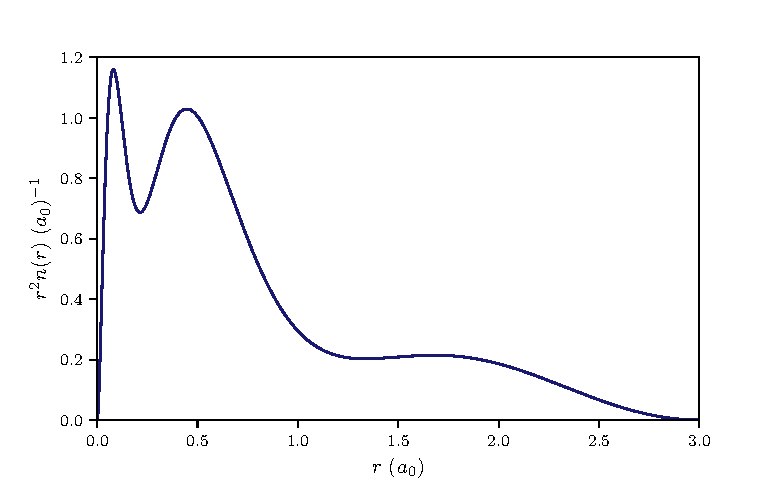
\includegraphics{figures/density_example.pdf} 
\label{Al:dens_example} 
\caption{Radial density distribution $r^2 n(r)$ for Aluminium at                     its solid density $\rho_\textrm{m}=2.7\ \textrm{g cm}^{-3}$ and                     temperature $T = 0.01\ \textrm{eV}$, for the Dirichlet                     boundary condition.} 
\end{figure}    \end{center}
    { \hspace*{\fill} \\}
    
    \hypertarget{convergence-testing}{%
\subsection{Convergence testing}\label{convergence-testing}}

There are various parameters which should be checked for convergence.
For all the boundary conditions, the main ones are:

\begin{itemize}
\tightlist
\item
  \texttt{nmax}: the maximum number of the principal quantum number
  \(n\)
\item
  \texttt{lmax}: the maximum number of the angular quantum number \(l\)
\item
  \texttt{grid\_params}: dictionary parameter controlling the
  logarithmic grid, in particular the number of grid points
  \texttt{ngrid}
\end{itemize}

Furthermore, for the \texttt{bands} boundary condition, there is the
additional dictionary parameter \texttt{band\_params}. The important
property within this is \texttt{nkpts} number of `k' points, which is
the number of states that are computed within all energy bands (spaced
linearly in energy) in our model.

The convergence for the \texttt{nmax} and \texttt{lmax} paramaters can
generally be chosen by eye, in other words by ensuring there are
sufficient states such that the highest levels have (nearly) zero
occoupations. Let us consider our Aluminium atom from earlier, but now
we shall increase the temperature (so more orbitals are required).

    \begin{tcolorbox}[breakable, size=fbox, boxrule=1pt, pad at break*=1mm,colback=cellbackground, colframe=cellborder]
\prompt{In}{incolor}{6}{\boxspacing}
\begin{Verbatim}[commandchars=\\\{\}]
\PY{c+c1}{\PYZsh{} set the temperature to 10 eV}
\PY{n}{Al\PYZus{}atom}\PY{o}{.}\PY{n}{units\PYZus{}temp} \PY{o}{=} \PY{l+s+s2}{\PYZdq{}}\PY{l+s+s2}{eV}\PY{l+s+s2}{\PYZdq{}}
\PY{n}{Al\PYZus{}atom}\PY{o}{.}\PY{n}{temp} \PY{o}{=} \PY{l+m+mi}{10}

\PY{c+c1}{\PYZsh{} run the calculation again}
\PY{n}{output} \PY{o}{=} \PY{n}{Al\PYZus{}model}\PY{o}{.}\PY{n}{CalcEnergy}\PY{p}{(}\PY{n}{nmax}\PY{p}{,} \PY{n}{lmax}\PY{p}{,} \PY{n}{write\PYZus{}info}\PY{o}{=}\PY{k+kc}{True}\PY{p}{)}
\end{Verbatim}
\end{tcolorbox}

    \begin{Verbatim}[commandchars=\\\{\}]
Starting SCF energy calculation

iscf   E\_free (Ha)    dE (1.0e-05)   dn (1.0e-04)   dv (1.0e-04)
-----------------------------------------------------------------
   0   -214.2613678      1.000e+00      9.999e-01      1.000e+00
   1   -224.1287430      4.403e-02      1.020e+00      7.395e-01
   2   -237.0838124      5.464e-02      8.010e-01      4.294e-01
   3   -242.4343199      2.207e-02      2.026e-01      6.883e-02
   4   -242.5475915      4.670e-04      3.594e-02      1.508e-02
   5   -242.5491121      6.269e-06      3.520e-03      6.318e-03
   6   -242.5492575      5.992e-07      1.319e-03      2.665e-03
   7   -242.5492674      4.081e-08      4.664e-04      1.134e-03
   8   -242.5492662      4.693e-09      1.654e-04      4.839e-04
   9   -242.5492654      3.390e-09      5.894e-05      2.061e-04
  10   -242.5492651      1.177e-09      2.111e-05      8.756e-05
-----------------------------------------------------------------
SCF cycle converged

Final energies (Ha)

---------------------------------------------
Kinetic energy                 :   245.0512
    orbitals                   :   245.0512
    unbound ideal approx.      :     0.0000
Electron-nuclear energy        :  -585.8430
Hartree energy                 :   119.0002
Exchange-correlation energy    :   -17.9878
    exchange                   :   -16.9823
    correlation                :    -1.0056
---------------------------------------------
Total energy                   :  -239.7795
---------------------------------------------
Entropy                        :     7.5369
    orbitals                   :     7.5369
    unbound ideal approx.      :     0.0000
---------------------------------------------
Total free energy              :  -242.5493
---------------------------------------------

Chemical potential             :   0.233
Mean ionization state          :   3.011

Orbital eigenvalues (Ha) :

     |   n=l+1 |       2 |       3 |       4 |       5
-----+---------+---------+---------+---------+---------
 l=0 | -54.614 |  -3.469 |   0.351 |   2.916 |   6.870
   1 |  -2.095 |   0.695 |   3.185 |   6.944 |  11.902
   2 |   1.115 |   3.241 |   6.500 |  10.930 |  16.512


Orbital occupations (2l+1) * f\_\{nl\} :

     |   n=l+1 |       2 |       3 |       4 |       5
-----+---------+---------+---------+---------+---------
 l=0 |   2.000 |   2.000 |   0.841 |   0.001 |   0.000
   1 |   5.989 |   1.330 |   0.002 |   0.000 |   0.000
   2 |   0.834 |   0.003 |   0.000 |   0.000 |   0.000


func:'CalcEnergy' took: 18.7312 sec
    \end{Verbatim}

    In the above example, we see that \texttt{nmax=5} seems to be
sufficiently large, but \texttt{lmax=3} is not, because the occupation
of the \(l=2,n=0\) state is 0.834, i.e.~significantly above zero. We
therefore choose a much larger value of \texttt{lmax} to check what is
required for convergence.

Since the diagonalization must be performed separately for every value
of \(0\leq l<\textrm{lmax}\), the computational time is proportional to
\texttt{lmax}. There is a simple kind of parallelization implemented in
atoMEC, courtesy of the joblib library \cite{joblib}, which parallelizes
the calculation over \texttt{l} (and also spin if
\texttt{model.spinpol=True}) and thus makes calculations more efficient.
This is enabled by the \texttt{config.numcores} parameter. Setting
\texttt{config.numcores=n} uses \texttt{n} cores; however, it is often
easiest to set \texttt{config.numcores=-1} which uses all the available
cores.

    \begin{tcolorbox}[breakable, size=fbox, boxrule=1pt, pad at break*=1mm,colback=cellbackground, colframe=cellborder]
\prompt{In}{incolor}{7}{\boxspacing}
\begin{Verbatim}[commandchars=\\\{\}]
\PY{c+c1}{\PYZsh{} enable parallelization}
\PY{k+kn}{from} \PY{n+nn}{atoMEC} \PY{k+kn}{import} \PY{n}{config}
\PY{n}{config}\PY{o}{.}\PY{n}{numcores} \PY{o}{=} \PY{o}{\PYZhy{}}\PY{l+m+mi}{1}

\PY{c+c1}{\PYZsh{} re\PYZhy{}run the calculation with larger lmax}
\PY{n}{lmax} \PY{o}{=} \PY{l+m+mi}{10}
\PY{n}{output} \PY{o}{=} \PY{n}{Al\PYZus{}model}\PY{o}{.}\PY{n}{CalcEnergy}\PY{p}{(}\PY{n}{nmax}\PY{p}{,} \PY{n}{lmax}\PY{p}{)}
\end{Verbatim}
\end{tcolorbox}

    \begin{Verbatim}[commandchars=\\\{\}]
Starting SCF energy calculation

iscf   E\_free (Ha)    dE (1.0e-05)   dn (1.0e-04)   dv (1.0e-04)
-----------------------------------------------------------------
   0   -214.2614028      1.000e+00      9.999e-01      1.000e+00
   1   -223.8611104      4.288e-02      1.026e+00      7.419e-01
   2   -237.0092438      5.548e-02      8.081e-01      4.366e-01
   3   -242.4583199      2.247e-02      2.045e-01      7.033e-02
   4   -242.5739605      4.767e-04      3.631e-02      1.568e-02
   5   -242.5755328      6.482e-06      3.614e-03      6.271e-03
   6   -242.5765476      4.183e-06      1.354e-03      2.642e-03
   7   -242.5765568      3.804e-08      4.785e-04      1.125e-03
   8   -242.5765553      6.421e-09      1.698e-04      4.803e-04
   9   -242.5765543      4.062e-09      6.050e-05      2.048e-04
  10   -242.5765065      1.968e-07      2.610e-05      4.115e-04
  11   -242.5765539      1.954e-07      2.242e-05      3.311e-04
  12   -242.5765539      3.520e-10      2.819e-06      1.340e-04
  13   -242.5765538      1.185e-10      1.014e-06      5.416e-05
-----------------------------------------------------------------
SCF cycle converged

Final energies (Ha)

---------------------------------------------
Kinetic energy                 :   245.1078
    orbitals                   :   245.1078
    unbound ideal approx.      :     0.0000
Electron-nuclear energy        :  -585.7124
Hartree energy                 :   118.9167
Exchange-correlation energy    :   -17.9809
    exchange                   :   -16.9756
    correlation                :    -1.0053
---------------------------------------------
Total energy                   :  -239.6687
---------------------------------------------
Entropy                        :     7.9127
    orbitals                   :     7.9127
    unbound ideal approx.      :     0.0000
---------------------------------------------
Total free energy              :  -242.5766
---------------------------------------------

Chemical potential             :   0.219
Mean ionization state          :   3.011

Orbital eigenvalues (Ha) :

     |   n=l+1 |       2 |       3 |       4 |       5
-----+---------+---------+---------+---------+---------
 l=0 | -54.624 |  -3.476 |   0.349 |   2.913 |   6.867
   1 |  -2.102 |   0.692 |   3.182 |   6.941 |  11.898
   2 |   1.112 |   3.237 |   6.496 |  10.926 |  16.508
   3 |   2.168 |   5.108 |   9.102 |  14.205 |  20.430
   4 |   3.254 |   6.876 |  11.538 |  17.284 |  24.134
   5 |   4.446 |   8.710 |  14.004 |  20.368 |  27.825
   6 |   5.758 |  10.653 |  16.560 |  23.529 |  31.580
   7 |   7.195 |  12.718 |  19.232 |  26.796 |  35.436


Orbital occupations (2l+1) * f\_\{nl\} :

     |   n=l+1 |       2 |       3 |       4 |       5
-----+---------+---------+---------+---------+---------
 l=0 |   2.000 |   2.000 |   0.825 |   0.001 |   0.000
   1 |   5.989 |   1.297 |   0.002 |   0.000 |   0.000
   2 |   0.809 |   0.003 |   0.000 |   0.000 |   0.000
   3 |   0.069 |   0.000 |   0.000 |   0.000 |   0.000
   4 |   0.005 |   0.000 |   0.000 |   0.000 |   0.000
   5 |   0.000 |   0.000 |   0.000 |   0.000 |   0.000
   6 |   0.000 |   0.000 |   0.000 |   0.000 |   0.000
   7 |   0.000 |   0.000 |   0.000 |   0.000 |   0.000


func:'CalcEnergy' took: 19.9555 sec
    \end{Verbatim}

    In the above, we clearly see that \texttt{lmax=10} is more than
sufficient; in fact, it seems that \texttt{lmax=6} is enough in this
case. Next, we shall test the convergence with respect to the number of
grid points. We suppress the output from the SCF cycle since we shall
run several calculations. If you are running this notebook, be patient
as running all the calculations will take some time.

    \begin{tcolorbox}[breakable, size=fbox, boxrule=1pt, pad at break*=1mm,colback=cellbackground, colframe=cellborder]
\prompt{In}{incolor}{8}{\boxspacing}
\begin{Verbatim}[commandchars=\\\{\}]
\PY{c+c1}{\PYZsh{} set up the grid points to test over}
\PY{n}{ngrid\PYZus{}test} \PY{o}{=} \PY{n}{np}\PY{o}{.}\PY{n}{arange}\PY{p}{(}\PY{l+m+mi}{500}\PY{p}{,} \PY{l+m+mi}{4500}\PY{p}{,} \PY{l+m+mi}{500}\PY{p}{)}

\PY{c+c1}{\PYZsh{} set up array to store the total energy, 1s core energy and chemical potential}
\PY{n}{output\PYZus{}arr} \PY{o}{=} \PY{n}{np}\PY{o}{.}\PY{n}{zeros}\PY{p}{(}\PY{p}{(}\PY{n+nb}{len}\PY{p}{(}\PY{n}{ngrid\PYZus{}test}\PY{p}{)}\PY{p}{,} \PY{l+m+mi}{4}\PY{p}{)}\PY{p}{)}

\PY{c+c1}{\PYZsh{} reset lmax to 6}
\PY{n}{lmax} \PY{o}{=} \PY{l+m+mi}{6}

\PY{c+c1}{\PYZsh{} change into the converence directory}
\PY{n}{os}\PY{o}{.}\PY{n}{chdir}\PY{p}{(}\PY{n}{basedir} \PY{o}{+} \PY{l+s+s2}{\PYZdq{}}\PY{l+s+s2}{/convergence\PYZus{}tests/}\PY{l+s+s2}{\PYZdq{}}\PY{p}{)}
\PY{c+c1}{\PYZsh{} loop over the ngrid array}
\PY{k}{for} \PY{n}{i}\PY{p}{,} \PY{n}{ngrid} \PY{o+ow}{in} \PY{n+nb}{enumerate}\PY{p}{(}\PY{n}{ngrid\PYZus{}test}\PY{p}{)}\PY{p}{:}
    \PY{c+c1}{\PYZsh{} set the output to an external file}
    \PY{n}{sys}\PY{o}{.}\PY{n}{stdout} \PY{o}{=} \PY{n+nb}{open}\PY{p}{(}\PY{l+s+s2}{\PYZdq{}}\PY{l+s+s2}{Al\PYZus{}ngrid\PYZus{}}\PY{l+s+s2}{\PYZdq{}} \PY{o}{+} \PY{n+nb}{str}\PY{p}{(}\PY{n}{ngrid}\PY{p}{)} \PY{o}{+} \PY{l+s+s2}{\PYZdq{}}\PY{l+s+s2}{.log}\PY{l+s+s2}{\PYZdq{}}\PY{p}{,} \PY{l+s+s2}{\PYZdq{}}\PY{l+s+s2}{w}\PY{l+s+s2}{\PYZdq{}}\PY{p}{)}
    \PY{n}{output} \PY{o}{=} \PY{n}{Al\PYZus{}model}\PY{o}{.}\PY{n}{CalcEnergy}\PY{p}{(}
        \PY{n}{nmax}\PY{p}{,} \PY{n}{lmax}\PY{p}{,} \PY{n}{grid\PYZus{}params}\PY{o}{=}\PY{p}{\PYZob{}}\PY{l+s+s2}{\PYZdq{}}\PY{l+s+s2}{ngrid}\PY{l+s+s2}{\PYZdq{}}\PY{p}{:} \PY{n}{ngrid}\PY{p}{\PYZcb{}}\PY{p}{,} \PY{n}{write\PYZus{}info}\PY{o}{=}\PY{k+kc}{False}
    \PY{p}{)}
    \PY{n}{output\PYZus{}arr}\PY{p}{[}\PY{n}{i}\PY{p}{,} \PY{l+m+mi}{0}\PY{p}{]} \PY{o}{=} \PY{n}{ngrid}
    \PY{n}{output\PYZus{}arr}\PY{p}{[}\PY{n}{i}\PY{p}{,} \PY{l+m+mi}{1}\PY{p}{]} \PY{o}{=} \PY{n}{output}\PY{p}{[}\PY{l+s+s2}{\PYZdq{}}\PY{l+s+s2}{energy}\PY{l+s+s2}{\PYZdq{}}\PY{p}{]}\PY{o}{.}\PY{n}{F\PYZus{}tot}
    \PY{n}{output\PYZus{}arr}\PY{p}{[}\PY{n}{i}\PY{p}{,} \PY{l+m+mi}{2}\PY{p}{]} \PY{o}{=} \PY{n}{output}\PY{p}{[}\PY{l+s+s2}{\PYZdq{}}\PY{l+s+s2}{orbitals}\PY{l+s+s2}{\PYZdq{}}\PY{p}{]}\PY{o}{.}\PY{n}{eigvals}\PY{p}{[}\PY{l+m+mi}{0}\PY{p}{,} \PY{l+m+mi}{0}\PY{p}{,} \PY{l+m+mi}{0}\PY{p}{,} \PY{l+m+mi}{0}\PY{p}{]}
    \PY{n}{output\PYZus{}arr}\PY{p}{[}\PY{n}{i}\PY{p}{,} \PY{l+m+mi}{3}\PY{p}{]} \PY{o}{=} \PY{n}{config}\PY{o}{.}\PY{n}{mu}

\PY{n}{os}\PY{o}{.}\PY{n}{chdir}\PY{p}{(}\PY{n}{basedir}\PY{p}{)} \PY{c+c1}{\PYZsh{} change back to base directory}
\PY{n}{sys}\PY{o}{.}\PY{n}{stdout} \PY{o}{=} \PY{n}{default\PYZus{}stdout} \PY{c+c1}{\PYZsh{} change output back to console}
\end{Verbatim}
\end{tcolorbox}

    We tabulate the total energy, core \(1s\) energy level and chemical
potential \(\mu\) below to check their convergence with respect to the
grid size.

    \begin{tcolorbox}[breakable, size=fbox, boxrule=1pt, pad at break*=1mm,colback=cellbackground, colframe=cellborder]
\prompt{In}{incolor}{9}{\boxspacing}
\begin{Verbatim}[commandchars=\\\{\}]
\PY{c+c1}{\PYZsh{} import package to make nice tables}
\PY{k+kn}{import} \PY{n+nn}{tabulate}

\PY{c+c1}{\PYZsh{} define table headings}
\PY{n}{headers} \PY{o}{=} \PY{p}{[}\PY{l+s+s2}{\PYZdq{}}\PY{l+s+s2}{ngrid}\PY{l+s+s2}{\PYZdq{}}\PY{p}{,} \PY{l+s+s2}{\PYZdq{}}\PY{l+s+s2}{F tot}\PY{l+s+s2}{\PYZdq{}}\PY{p}{,} \PY{l+s+s2}{\PYZdq{}}\PY{l+s+s2}{e\PYZus{}1s}\PY{l+s+s2}{\PYZdq{}}\PY{p}{,} \PY{l+s+s2}{\PYZdq{}}\PY{l+s+s2}{mu}\PY{l+s+s2}{\PYZdq{}}\PY{p}{]}

\PY{c+c1}{\PYZsh{} create table}
\PY{n}{conv\PYZus{}tbl} \PY{o}{=} \PY{n}{tabulate}\PY{o}{.}\PY{n}{tabulate}\PY{p}{(}
    \PY{n}{output\PYZus{}arr}\PY{p}{,}
    \PY{n}{headers}\PY{p}{,}
    \PY{n}{tablefmt}\PY{o}{=}\PY{l+s+s2}{\PYZdq{}}\PY{l+s+s2}{presto}\PY{l+s+s2}{\PYZdq{}}\PY{p}{,}
    \PY{n}{floatfmt}\PY{o}{=}\PY{p}{[}\PY{l+s+s2}{\PYZdq{}}\PY{l+s+s2}{4.0f}\PY{l+s+s2}{\PYZdq{}}\PY{p}{,} \PY{l+s+s2}{\PYZdq{}}\PY{l+s+s2}{7.3f}\PY{l+s+s2}{\PYZdq{}}\PY{p}{,} \PY{l+s+s2}{\PYZdq{}}\PY{l+s+s2}{7.3f}\PY{l+s+s2}{\PYZdq{}}\PY{p}{,} \PY{l+s+s2}{\PYZdq{}}\PY{l+s+s2}{7.3f}\PY{l+s+s2}{\PYZdq{}}\PY{p}{]}\PY{p}{,}
    \PY{n}{stralign}\PY{o}{=}\PY{l+s+s2}{\PYZdq{}}\PY{l+s+s2}{right}\PY{l+s+s2}{\PYZdq{}}\PY{p}{,}
\PY{p}{)}
\PY{n+nb}{print}\PY{p}{(}\PY{n}{conv\PYZus{}tbl}\PY{p}{)}
\end{Verbatim}
\end{tcolorbox}

    \begin{Verbatim}[commandchars=\\\{\}]
   ngrid |    F tot |    e\_1s |      mu
---------+----------+---------+---------
     500 | -243.265 | -54.713 |   0.189
    1000 | -242.576 | -54.623 |   0.219
    1500 | -242.345 | -54.595 |   0.229
    2000 | -242.229 | -54.580 |   0.235
    2500 | -242.159 | -54.572 |   0.238
    3000 | -242.113 | -54.566 |   0.240
    3500 | -242.080 | -54.561 |   0.242
    4000 | -242.055 | -54.559 |   0.242
    \end{Verbatim}

    The degree of convergence required depends on various factors, such as
the error that the user is willing to tolerate and the property that is
being computed. In AA models, there are already a number of quite
serious approximations which create uncertainty in the results, so
typically we can use more relaxed convergence criteria than a full
DFT-MD simulation. The property we are interested in for the purposes of
this paper is the MIS, which is sensitive to the energy eigenvalues and
chemical potential but not the total energy. Furthermore, we aim to
benchmark our results agaist experiments which of course have some
uncertainty for measurements of the free electron density.

With the above factors taken into account, we typically aim for
convergence of around \(0.01\ \textrm{Ha}\) in the core \(1s\) energy
level and the chemical potential \(\mu\). Based on the above table, this
indicates a reasonable choice is \texttt{ngrid=3000}. In theory, this
number should be checked for each value of temperature and density
calculated. In practise, it is reasonable to test it for a few select
values in the temperature or density range spanned and interpolate to
the other values.

As mentioned, when the \texttt{bands} boundary condition is used, we
must also test convergence with respect to the number of orbitals
\texttt{nkpts} per band. We perform a similar convergence check to
before, only now we shall we probe the lowest energy eigenvalue in the
conduction band, instead of the \(1s\) core energy level. This is
because, under these conditions, the \(1s\) level is fully isolated from
the neighbouring spheres and so is not part of an energy band.

    \begin{tcolorbox}[breakable, size=fbox, boxrule=1pt, pad at break*=1mm,colback=cellbackground, colframe=cellborder]
\prompt{In}{incolor}{10}{\boxspacing}
\begin{Verbatim}[commandchars=\\\{\}]
\PY{c+c1}{\PYZsh{} set up the nkpts array}
\PY{n}{nkpts\PYZus{}arr} \PY{o}{=} \PY{n}{np}\PY{o}{.}\PY{n}{arange}\PY{p}{(}\PY{l+m+mi}{10}\PY{p}{,} \PY{l+m+mi}{110}\PY{p}{,} \PY{l+m+mi}{10}\PY{p}{)}

\PY{c+c1}{\PYZsh{} change the boundary condition}
\PY{n}{Al\PYZus{}model}\PY{o}{.}\PY{n}{bc} \PY{o}{=} \PY{l+s+s2}{\PYZdq{}}\PY{l+s+s2}{bands}\PY{l+s+s2}{\PYZdq{}}

\PY{c+c1}{\PYZsh{} reset the output array}
\PY{n}{output\PYZus{}arr} \PY{o}{=} \PY{n}{np}\PY{o}{.}\PY{n}{zeros}\PY{p}{(}\PY{p}{(}\PY{n+nb}{len}\PY{p}{(}\PY{n}{nkpts\PYZus{}arr}\PY{p}{)}\PY{p}{,} \PY{l+m+mi}{4}\PY{p}{)}\PY{p}{)}

\PY{c+c1}{\PYZsh{} change to convergence directory}
\PY{n}{os}\PY{o}{.}\PY{n}{chdir}\PY{p}{(}\PY{n}{basedir} \PY{o}{+} \PY{l+s+s2}{\PYZdq{}}\PY{l+s+s2}{/convergence\PYZus{}tests/}\PY{l+s+s2}{\PYZdq{}}\PY{p}{)}
\PY{c+c1}{\PYZsh{} loop over the nkpts array with a coarse ngrid value (independent)}
\PY{k}{for} \PY{n}{i}\PY{p}{,} \PY{n}{nkpts} \PY{o+ow}{in} \PY{n+nb}{enumerate}\PY{p}{(}\PY{n}{nkpts\PYZus{}arr}\PY{p}{)}\PY{p}{:}
    \PY{c+c1}{\PYZsh{} set the output to an external file}
    \PY{n}{sys}\PY{o}{.}\PY{n}{stdout} \PY{o}{=} \PY{n+nb}{open}\PY{p}{(}\PY{l+s+s2}{\PYZdq{}}\PY{l+s+s2}{Al\PYZus{}nkpts\PYZus{}}\PY{l+s+s2}{\PYZdq{}} \PY{o}{+} \PY{n+nb}{str}\PY{p}{(}\PY{n}{ngrid}\PY{p}{)} \PY{o}{+} \PY{l+s+s2}{\PYZdq{}}\PY{l+s+s2}{.log}\PY{l+s+s2}{\PYZdq{}}\PY{p}{,} \PY{l+s+s2}{\PYZdq{}}\PY{l+s+s2}{w}\PY{l+s+s2}{\PYZdq{}}\PY{p}{)}
    \PY{n}{output} \PY{o}{=} \PY{n}{Al\PYZus{}model}\PY{o}{.}\PY{n}{CalcEnergy}\PY{p}{(}
        \PY{n}{nmax}\PY{p}{,}
        \PY{n}{lmax}\PY{p}{,}
        \PY{n}{grid\PYZus{}params}\PY{o}{=}\PY{p}{\PYZob{}}\PY{l+s+s2}{\PYZdq{}}\PY{l+s+s2}{ngrid}\PY{l+s+s2}{\PYZdq{}}\PY{p}{:} \PY{l+m+mi}{1000}\PY{p}{\PYZcb{}}\PY{p}{,}
        \PY{n}{write\PYZus{}info}\PY{o}{=}\PY{k+kc}{False}\PY{p}{,}
        \PY{n}{band\PYZus{}params}\PY{o}{=}\PY{p}{\PYZob{}}\PY{l+s+s2}{\PYZdq{}}\PY{l+s+s2}{nkpts}\PY{l+s+s2}{\PYZdq{}}\PY{p}{:} \PY{n}{nkpts}\PY{p}{\PYZcb{}}\PY{p}{,}
    \PY{p}{)}
    \PY{n}{output\PYZus{}arr}\PY{p}{[}\PY{n}{i}\PY{p}{,} \PY{l+m+mi}{0}\PY{p}{]} \PY{o}{=} \PY{n}{nkpts}
    \PY{n}{output\PYZus{}arr}\PY{p}{[}\PY{n}{i}\PY{p}{,} \PY{l+m+mi}{1}\PY{p}{]} \PY{o}{=} \PY{n}{output}\PY{p}{[}\PY{l+s+s2}{\PYZdq{}}\PY{l+s+s2}{energy}\PY{l+s+s2}{\PYZdq{}}\PY{p}{]}\PY{o}{.}\PY{n}{F\PYZus{}tot}
    \PY{n}{output\PYZus{}arr}\PY{p}{[}\PY{n}{i}\PY{p}{,} \PY{l+m+mi}{2}\PY{p}{]} \PY{o}{=} \PY{n}{output}\PY{p}{[}\PY{l+s+s2}{\PYZdq{}}\PY{l+s+s2}{orbitals}\PY{l+s+s2}{\PYZdq{}}\PY{p}{]}\PY{o}{.}\PY{n}{eigvals}\PY{p}{[}\PY{l+m+mi}{0}\PY{p}{,} \PY{l+m+mi}{0}\PY{p}{,} \PY{l+m+mi}{0}\PY{p}{,} \PY{l+m+mi}{2}\PY{p}{]}
    \PY{n}{output\PYZus{}arr}\PY{p}{[}\PY{n}{i}\PY{p}{,} \PY{l+m+mi}{3}\PY{p}{]} \PY{o}{=} \PY{n}{config}\PY{o}{.}\PY{n}{mu}
    
\PY{n}{os}\PY{o}{.}\PY{n}{chdir}\PY{p}{(}\PY{n}{basedir}\PY{p}{)} \PY{c+c1}{\PYZsh{} change back to base directory}
\PY{n}{sys}\PY{o}{.}\PY{n}{stdout} \PY{o}{=} \PY{n}{default\PYZus{}stdout} \PY{c+c1}{\PYZsh{} change output back to console}
\end{Verbatim}
\end{tcolorbox}

    \begin{tcolorbox}[breakable, size=fbox, boxrule=1pt, pad at break*=1mm,colback=cellbackground, colframe=cellborder]
\prompt{In}{incolor}{11}{\boxspacing}
\begin{Verbatim}[commandchars=\\\{\}]
\PY{c+c1}{\PYZsh{} create table}
\PY{n}{headers} \PY{o}{=} \PY{p}{[}\PY{l+s+s2}{\PYZdq{}}\PY{l+s+s2}{nkpts}\PY{l+s+s2}{\PYZdq{}}\PY{p}{,} \PY{l+s+s2}{\PYZdq{}}\PY{l+s+s2}{F tot}\PY{l+s+s2}{\PYZdq{}}\PY{p}{,} \PY{l+s+s2}{\PYZdq{}}\PY{l+s+s2}{e\PYZus{}c}\PY{l+s+s2}{\PYZdq{}}\PY{p}{,} \PY{l+s+s2}{\PYZdq{}}\PY{l+s+s2}{mu}\PY{l+s+s2}{\PYZdq{}}\PY{p}{]}
\PY{n}{conv\PYZus{}tbl} \PY{o}{=} \PY{n}{tabulate}\PY{o}{.}\PY{n}{tabulate}\PY{p}{(}
    \PY{n}{output\PYZus{}arr}\PY{p}{,}
    \PY{n}{headers}\PY{p}{,}
    \PY{n}{tablefmt}\PY{o}{=}\PY{l+s+s2}{\PYZdq{}}\PY{l+s+s2}{presto}\PY{l+s+s2}{\PYZdq{}}\PY{p}{,}
    \PY{n}{floatfmt}\PY{o}{=}\PY{p}{[}\PY{l+s+s2}{\PYZdq{}}\PY{l+s+s2}{4.0f}\PY{l+s+s2}{\PYZdq{}}\PY{p}{,} \PY{l+s+s2}{\PYZdq{}}\PY{l+s+s2}{7.3f}\PY{l+s+s2}{\PYZdq{}}\PY{p}{,} \PY{l+s+s2}{\PYZdq{}}\PY{l+s+s2}{7.3f}\PY{l+s+s2}{\PYZdq{}}\PY{p}{,} \PY{l+s+s2}{\PYZdq{}}\PY{l+s+s2}{7.3f}\PY{l+s+s2}{\PYZdq{}}\PY{p}{]}\PY{p}{,}
    \PY{n}{stralign}\PY{o}{=}\PY{l+s+s2}{\PYZdq{}}\PY{l+s+s2}{right}\PY{l+s+s2}{\PYZdq{}}\PY{p}{,}
\PY{p}{)}
\PY{n+nb}{print}\PY{p}{(}\PY{n}{conv\PYZus{}tbl}\PY{p}{)}
\end{Verbatim}
\end{tcolorbox}

    \begin{Verbatim}[commandchars=\\\{\}]
   nkpts |    F tot |     e\_c |      mu
---------+----------+---------+---------
      10 | -243.814 |  -0.131 |  -0.038
      20 | -243.859 |  -0.130 |  -0.053
      30 | -243.869 |  -0.130 |  -0.057
      40 | -243.873 |  -0.130 |  -0.058
      50 | -243.875 |  -0.130 |  -0.059
      60 | -243.877 |  -0.130 |  -0.059
      70 | -243.878 |  -0.130 |  -0.059
      80 | -243.878 |  -0.130 |  -0.059
      90 | -243.879 |  -0.130 |  -0.060
     100 | -243.879 |  -0.130 |  -0.060
    \end{Verbatim}

    We see from the above that, for this example, the quantities of interest
are very well converged already with \texttt{nkpts=20}. However, the
time taken is almost identical regardless of the number of \(k\)-points
used. This is because the computationally dominant step is actually the
diagonalization of the Hamiltonian, which is required to find the limits
of the band energies. Therefore we are free to choose a relatively large
value of \texttt{nkpts} without much affect on the computational
demands. Typically the default value of \texttt{nkpts=50} in atoMEC is a
reasonable choice.

    \hypertarget{density-of-states-for-carbon-with-aa-model}{%
\section{Density-of-states for Carbon with AA
model}\label{density-of-states-for-carbon-with-aa-model}}

We shall now calculate and plot the DOS for Carbon using the
band-structure AA model under a range of densities, for temperature
\(T=100\ \textrm{eV}\). The conditions we use are identical to those
considered in Ref. \onlinecite{Redmer_Kubo_Greenwood}, in order to
facilitate comparison between the AA model and a full DFT-MD simulation.

First, we calculate the DOS for Carbon under these conditions:

    \begin{tcolorbox}[breakable, size=fbox, boxrule=1pt, pad at break*=1mm,colback=cellbackground, colframe=cellborder]
\prompt{In}{incolor}{12}{\boxspacing}
\begin{Verbatim}[commandchars=\\\{\}]
\PY{c+c1}{\PYZsh{} set up the base Carbon atom}
\PY{n}{C\PYZus{}atom} \PY{o}{=} \PY{n}{Atom}\PY{p}{(}\PY{l+s+s2}{\PYZdq{}}\PY{l+s+s2}{C}\PY{l+s+s2}{\PYZdq{}}\PY{p}{,} \PY{l+m+mi}{100}\PY{p}{,} \PY{n}{density}\PY{o}{=}\PY{l+m+mf}{1.0}\PY{p}{,} \PY{n}{units\PYZus{}temp}\PY{o}{=}\PY{l+s+s2}{\PYZdq{}}\PY{l+s+s2}{eV}\PY{l+s+s2}{\PYZdq{}}\PY{p}{,} \PY{n}{write\PYZus{}info}\PY{o}{=}\PY{k+kc}{False}\PY{p}{)}
\PY{c+c1}{\PYZsh{} set up the base model}
\PY{n}{model} \PY{o}{=} \PY{n}{models}\PY{o}{.}\PY{n}{ISModel}\PY{p}{(}\PY{n}{C\PYZus{}atom}\PY{p}{,} \PY{n}{unbound}\PY{o}{=}\PY{l+s+s2}{\PYZdq{}}\PY{l+s+s2}{quantum}\PY{l+s+s2}{\PYZdq{}}\PY{p}{,} \PY{n}{bc}\PY{o}{=}\PY{l+s+s2}{\PYZdq{}}\PY{l+s+s2}{bands}\PY{l+s+s2}{\PYZdq{}}\PY{p}{,} \PY{n}{write\PYZus{}info}\PY{o}{=}\PY{k+kc}{False}\PY{p}{)}
\PY{c+c1}{\PYZsh{} define the densities}
\PY{n}{densities} \PY{o}{=} \PY{n}{np}\PY{o}{.}\PY{n}{array}\PY{p}{(}\PY{p}{[}\PY{l+m+mi}{20}\PY{p}{,} \PY{l+m+mi}{30}\PY{p}{,} \PY{l+m+mi}{50}\PY{p}{,} \PY{l+m+mi}{80}\PY{p}{,} \PY{l+m+mi}{100}\PY{p}{,} \PY{l+m+mi}{150}\PY{p}{,} \PY{l+m+mi}{200}\PY{p}{,} \PY{l+m+mi}{300}\PY{p}{,} \PY{l+m+mi}{400}\PY{p}{]}\PY{p}{,} \PY{n}{dtype}\PY{o}{=}\PY{n+nb}{float}\PY{p}{)}
\PY{c+c1}{\PYZsh{} set up empty array of chemical potentials}
\PY{n}{chem\PYZus{}pots} \PY{o}{=} \PY{n}{np}\PY{o}{.}\PY{n}{zeros\PYZus{}like}\PY{p}{(}\PY{n}{densities}\PY{p}{)}
\PY{c+c1}{\PYZsh{} set the lmax and nmax parameters}
\PY{n}{lmax} \PY{o}{=} \PY{l+m+mi}{10}
\PY{n}{nmax} \PY{o}{=} \PY{l+m+mi}{10}
\PY{c+c1}{\PYZsh{} grid parameters}
\PY{n}{grid\PYZus{}params} \PY{o}{=} \PY{p}{\PYZob{}}\PY{l+s+s2}{\PYZdq{}}\PY{l+s+s2}{ngrid}\PY{l+s+s2}{\PYZdq{}}\PY{p}{:} \PY{l+m+mi}{2000}\PY{p}{\PYZcb{}}
\PY{c+c1}{\PYZsh{} band parameters}
\PY{n}{band\PYZus{}params} \PY{o}{=} \PY{p}{\PYZob{}}\PY{l+s+s2}{\PYZdq{}}\PY{l+s+s2}{nkpts}\PY{l+s+s2}{\PYZdq{}}\PY{p}{:} \PY{l+m+mi}{50}\PY{p}{\PYZcb{}}

\PY{c+c1}{\PYZsh{} change into the bc directory}
\PY{n}{os}\PY{o}{.}\PY{n}{chdir}\PY{p}{(}\PY{n}{basedir} \PY{o}{+} \PY{l+s+s2}{\PYZdq{}}\PY{l+s+s2}{/results/Carbon/bands/}\PY{l+s+s2}{\PYZdq{}}\PY{p}{)}
\PY{k}{for} \PY{n}{i}\PY{p}{,} \PY{n}{density} \PY{o+ow}{in} \PY{n+nb}{enumerate}\PY{p}{(}\PY{n}{densities}\PY{p}{)}\PY{p}{:}
    \PY{c+c1}{\PYZsh{} set the output to an external file}
    \PY{n}{sys}\PY{o}{.}\PY{n}{stdout} \PY{o}{=} \PY{n+nb}{open}\PY{p}{(}\PY{l+s+s2}{\PYZdq{}}\PY{l+s+s2}{C\PYZus{}}\PY{l+s+s2}{\PYZdq{}} \PY{o}{+} \PY{n+nb}{str}\PY{p}{(}\PY{n}{density}\PY{p}{)} \PY{o}{+} \PY{l+s+s2}{\PYZdq{}}\PY{l+s+s2}{.log}\PY{l+s+s2}{\PYZdq{}}\PY{p}{,} \PY{l+s+s2}{\PYZdq{}}\PY{l+s+s2}{w}\PY{l+s+s2}{\PYZdq{}}\PY{p}{)}
    \PY{c+c1}{\PYZsh{} set the density}
    \PY{n}{C\PYZus{}atom}\PY{o}{.}\PY{n}{density} \PY{o}{=} \PY{n}{density}
    \PY{c+c1}{\PYZsh{} run the SCF calculation}
    \PY{n}{output} \PY{o}{=} \PY{n}{model}\PY{o}{.}\PY{n}{CalcEnergy}\PY{p}{(}
        \PY{n}{nmax}\PY{p}{,}
        \PY{n}{lmax}\PY{p}{,}
        \PY{n}{grid\PYZus{}params}\PY{o}{=}\PY{n}{grid\PYZus{}params}\PY{p}{,}
        \PY{n}{band\PYZus{}params}\PY{o}{=}\PY{n}{band\PYZus{}params}\PY{p}{,}
        \PY{n}{dos\PYZus{}file}\PY{o}{=}\PY{l+s+s2}{\PYZdq{}}\PY{l+s+s2}{dos\PYZus{}}\PY{l+s+s2}{\PYZdq{}} \PY{o}{+} \PY{n+nb}{str}\PY{p}{(}\PY{n}{density}\PY{p}{)} \PY{o}{+} \PY{l+s+s2}{\PYZdq{}}\PY{l+s+s2}{.csv}\PY{l+s+s2}{\PYZdq{}}\PY{p}{,}
    \PY{p}{)}
    \PY{c+c1}{\PYZsh{} save the chemical potential}
    \PY{n}{chem\PYZus{}pots}\PY{p}{[}\PY{n}{i}\PY{p}{]} \PY{o}{=} \PY{n}{config}\PY{o}{.}\PY{n}{mu}

\PY{n}{os}\PY{o}{.}\PY{n}{chdir}\PY{p}{(}\PY{n}{basedir}\PY{p}{)} \PY{c+c1}{\PYZsh{} change back to base directory}
\PY{n}{sys}\PY{o}{.}\PY{n}{stdout} \PY{o}{=} \PY{n}{default\PYZus{}stdout} \PY{c+c1}{\PYZsh{} change output back to console}
\end{Verbatim}
\end{tcolorbox}

    \begin{Verbatim}[commandchars=\\\{\}]
Warning: this input temperature is very high. Proceeding anyway, but results may

    \end{Verbatim}

    Next, we plot the DOS:

    \begin{tcolorbox}[breakable, size=fbox, boxrule=1pt, pad at break*=1mm,colback=cellbackground, colframe=cellborder]
\prompt{In}{incolor}{13}{\boxspacing}
\begin{Verbatim}[commandchars=\\\{\}]
\PY{k+kn}{import} \PY{n+nn}{MIS\PYZus{}plots}
\PY{n}{MIS\PYZus{}plots}\PY{o}{.}\PY{n}{plot\PYZus{}DOS}\PY{p}{(}\PY{n}{densities}\PY{p}{,} \PY{n}{chem\PYZus{}pots}\PY{p}{)}
\end{Verbatim}
\end{tcolorbox}

    \begin{center}
\begin{figure} 
\centering 
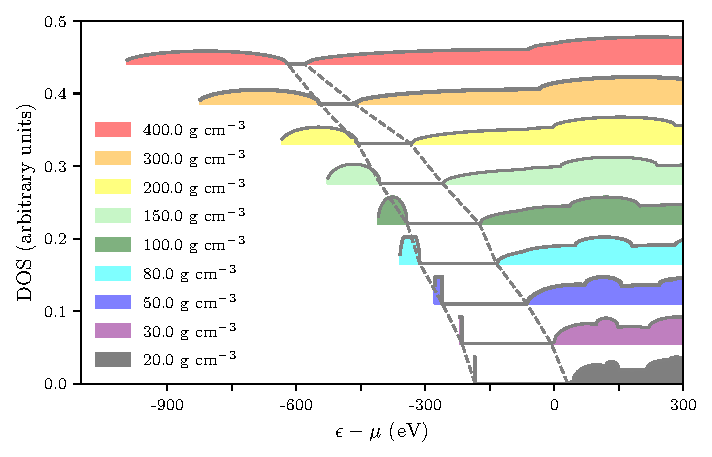
\includegraphics{figures/Carbon_DOS_comp.pdf} 
\label{C:dos_example} 
\caption{Density-of-states for Carbon at a range of densities                     and temperature $T = 100\ \textrm{eV}$, calculated with the AA                     band-structure model.} 
\end{figure}    \end{center}
    { \hspace*{\fill} \\}
    
    Note that, for the densities between \(20-80\ \textrm{g cm}^{-3}\), we
have truncated the peak of the part of the DOS that comes from the
valence (\(1s\)) band, because the band width approaches zero and thus
the DOS approaches a delta function. Nevertheless, the figure shows
strong qualitative agreeement with the equivalent Fig. 2 in Ref.
\onlinecite{Redmer_Kubo_Greenwood}; furthermore, the position and width
of the band gap is in quantitative agreement. This indicates the
band-structure AA model is a good approximation for the full DFT-MD
simulation under the above conditions.

    \hypertarget{mean-ionization-state-comparisons}{%
\section{Mean ionization state
comparisons}\label{mean-ionization-state-comparisons}}

In the previous section, we introduced the basics of running a
calculation in atoMEC to compute various quantities such as the KS
orbitals and the density. In this section, we explain how to compute the
MIS in atoMEC via the various methods described in the paper.
Afterwards, we provide the input (and output) for the calculations that
were done in the paper, so that the reader can reproduce these results.

\hypertarget{calculation-of-mis-using-the-threshold-method}{%
\subsection{Calculation of MIS using the threshold
method}\label{calculation-of-mis-using-the-threshold-method}}

As seen in Eq. (1) of the main paper, the MIS can be computed as the
integral over all the positive energy states:

\begin{equation}
\bar{Z} = \int_{v(R_\textrm{WS})}^\infty g(\epsilon) f_\textrm{FD}(\epsilon)\,,
\end{equation}

where \(g(\epsilon)\) is the density-of-states (DOS),
\(f_\textrm{FD}(\epsilon)\) the Fermi--Dirac distribution, and
\(v(R_\textrm{WS})\) the value of the potential at the Wigner--Seitz
(WS) radius.

In atoMEC, when \texttt{unbound="quantum"}, all the orbitals are treated
identically. The integral in the above equation therefore becomes a sum
over all the states with energies above \(v(R_\textrm{WS})\),

\begin{equation}
\bar{Z} = 2\sum_{k,\sigma,l,n} (2l+1) w_{k} f_{k ln} \Theta(\epsilon_{k ln}-v(R_\textrm{WS}))\,,
\end{equation}

where \(\Theta\) is the Heaviside step function.

As was seen in the earlier examples, the MIS calculate via the threshold
method is printed by default at the end of every SCF run anyway. It is
also a property of the \texttt{staticKS.Density} object so can be
accessed through that if desired. Let us again run a calculation for
Aluminium at ambient conditions:

    \begin{tcolorbox}[breakable, size=fbox, boxrule=1pt, pad at break*=1mm,colback=cellbackground, colframe=cellborder]
\prompt{In}{incolor}{21}{\boxspacing}
\begin{Verbatim}[commandchars=\\\{\}]
\PY{c+c1}{\PYZsh{} first set up and run a calculation}
\PY{c+c1}{\PYZsh{} set up the ISModel}
\PY{n}{Al\PYZus{}model} \PY{o}{=} \PY{n}{models}\PY{o}{.}\PY{n}{ISModel}\PY{p}{(}
    \PY{n}{Al\PYZus{}atom}\PY{p}{,}
    \PY{n}{bc}\PY{o}{=}\PY{l+s+s2}{\PYZdq{}}\PY{l+s+s2}{dirichlet}\PY{l+s+s2}{\PYZdq{}}\PY{p}{,}
    \PY{n}{unbound}\PY{o}{=}\PY{l+s+s2}{\PYZdq{}}\PY{l+s+s2}{quantum}\PY{l+s+s2}{\PYZdq{}}\PY{p}{,}
    \PY{n}{xfunc\PYZus{}id}\PY{o}{=}\PY{l+s+s2}{\PYZdq{}}\PY{l+s+s2}{lda\PYZus{}x}\PY{l+s+s2}{\PYZdq{}}\PY{p}{,}
    \PY{n}{cfunc\PYZus{}id}\PY{o}{=}\PY{l+s+s2}{\PYZdq{}}\PY{l+s+s2}{lda\PYZus{}c\PYZus{}pw}\PY{l+s+s2}{\PYZdq{}}\PY{p}{,}
    \PY{n}{write\PYZus{}info}\PY{o}{=}\PY{k+kc}{False}\PY{p}{,}
\PY{p}{)}

\PY{c+c1}{\PYZsh{} reset temperature and density}
\PY{n}{Al\PYZus{}atom}\PY{o}{.}\PY{n}{temp} \PY{o}{=} \PY{l+m+mf}{0.01}
\PY{n}{Al\PYZus{}atom}\PY{o}{.}\PY{n}{density} \PY{o}{=} \PY{l+m+mf}{2.7}

\PY{c+c1}{\PYZsh{} set the values of nmax and lmax}
\PY{n}{nmax} \PY{o}{=} \PY{l+m+mi}{5}
\PY{n}{lmax} \PY{o}{=} \PY{l+m+mi}{3}

\PY{c+c1}{\PYZsh{} run the SCF calculation}
\PY{n}{output} \PY{o}{=} \PY{n}{Al\PYZus{}model}\PY{o}{.}\PY{n}{CalcEnergy}\PY{p}{(}
    \PY{n}{nmax}\PY{p}{,}
    \PY{n}{lmax}\PY{p}{,}
    \PY{n}{scf\PYZus{}params}\PY{o}{=}\PY{p}{\PYZob{}}\PY{l+s+s2}{\PYZdq{}}\PY{l+s+s2}{mixfrac}\PY{l+s+s2}{\PYZdq{}}\PY{p}{:} \PY{l+m+mf}{0.6}\PY{p}{,} \PY{l+s+s2}{\PYZdq{}}\PY{l+s+s2}{maxscf}\PY{l+s+s2}{\PYZdq{}}\PY{p}{:} \PY{l+m+mi}{50}\PY{p}{\PYZcb{}}\PY{p}{,}
    \PY{n}{grid\PYZus{}params}\PY{o}{=}\PY{p}{\PYZob{}}\PY{l+s+s2}{\PYZdq{}}\PY{l+s+s2}{ngrid}\PY{l+s+s2}{\PYZdq{}}\PY{p}{:} \PY{l+m+mi}{2000}\PY{p}{\PYZcb{}}\PY{p}{,}
    \PY{n}{write\PYZus{}info}\PY{o}{=}\PY{k+kc}{False}\PY{p}{,}
\PY{p}{)}
\end{Verbatim}
\end{tcolorbox}

    \begin{Verbatim}[commandchars=\\\{\}]

func:'CalcEnergy' took: 25.3485 sec
    \end{Verbatim}

    \begin{tcolorbox}[breakable, size=fbox, boxrule=1pt, pad at break*=1mm,colback=cellbackground, colframe=cellborder]
\prompt{In}{incolor}{22}{\boxspacing}
\begin{Verbatim}[commandchars=\\\{\}]
\PY{c+c1}{\PYZsh{} extract the MIS}
\PY{n}{MIS} \PY{o}{=} \PY{n}{output}\PY{p}{[}\PY{l+s+s2}{\PYZdq{}}\PY{l+s+s2}{density}\PY{l+s+s2}{\PYZdq{}}\PY{p}{]}\PY{o}{.}\PY{n}{MIS}

\PY{c+c1}{\PYZsh{} print the 1st array element (only element in a spin unpolarized calculation)}
\PY{n+nb}{print}\PY{p}{(}\PY{l+s+s2}{\PYZdq{}}\PY{l+s+s2}{MIS = }\PY{l+s+s2}{\PYZdq{}}\PY{p}{,} \PY{n+nb}{round}\PY{p}{(}\PY{n}{MIS}\PY{p}{[}\PY{l+m+mi}{0}\PY{p}{]}\PY{p}{,} \PY{l+m+mi}{2}\PY{p}{)}\PY{p}{)}
\end{Verbatim}
\end{tcolorbox}

    \begin{Verbatim}[commandchars=\\\{\}]
MIS =  3.0
    \end{Verbatim}

    In this case, the MIS computed with the threshold approach is equal to
\(3.0\), which is the number of orbitals in the conduction band for
Aluminium at ambient conditions.

    \hypertarget{calculation-of-mis-using-the-electron-localization-function}{%
\subsection{Calculation of MIS using the electron localization
function}\label{calculation-of-mis-using-the-electron-localization-function}}

As seen in Eq. (4) of the main paper, the electron localization function
(ELF) is defined as

\begin{gather}
\textrm{ELF}(r) = \frac{1}{1+[D(\vec{r})/D_0(\vec{r})]^2}\,,\textrm{ with} \\
D(\vec{r}) = D_0(\vec{r}) - \frac{1}{9} \frac{|\nabla n(\vec{r})^2|}{n(\vec{r})} + \frac{1}{6}\nabla^2 n(\vec{r})\,, \textrm{ and} \\
D_0(\vec{r}) = \frac{3}{10}(3\pi^2)^{2/3} n^{5/3}(r)\,.
\end{gather}

For a spherically symmetric system, \(D_0(r)=D_0(\vec{r})\) and the
expression for \(D(r)\) becomes

\begin{equation}
D(r) = D_0(r) - \frac{1}{9} \frac{1}{n(r)} \left| \frac{\textrm{d}n(r)}{\textrm{d}r}\right|^2 + \frac{1}{6} \left(  \frac{2}{r} \frac{\textrm{d}n(r)}{\textrm{d}r} +  \frac{\textrm{d}^2 n(r)}{\textrm{d}r^2}\right)\,.
\end{equation}

In atoMEC the ELF is accessed through the
\texttt{postprocess.localization} module. In the following, we calculate
and plot the ELF for our Aluminium example.

    \begin{tcolorbox}[breakable, size=fbox, boxrule=1pt, pad at break*=1mm,colback=cellbackground, colframe=cellborder]
\prompt{In}{incolor}{23}{\boxspacing}
\begin{Verbatim}[commandchars=\\\{\}]
\PY{c+c1}{\PYZsh{} import localization module}
\PY{k+kn}{from} \PY{n+nn}{atoMEC}\PY{n+nn}{.}\PY{n+nn}{postprocess} \PY{k+kn}{import} \PY{n}{localization}

\PY{c+c1}{\PYZsh{} Set up the ELF object}
\PY{c+c1}{\PYZsh{} use the \PYZdq{}density\PYZdq{} version of the ELF (uses second order gradient expansion for KED)}

\PY{n}{ELF\PYZus{}Al} \PY{o}{=} \PY{n}{localization}\PY{o}{.}\PY{n}{ELFTools}\PY{p}{(}\PY{n}{output}\PY{p}{[}\PY{l+s+s2}{\PYZdq{}}\PY{l+s+s2}{orbitals}\PY{l+s+s2}{\PYZdq{}}\PY{p}{]}\PY{p}{,} \PY{n}{output}\PY{p}{[}\PY{l+s+s2}{\PYZdq{}}\PY{l+s+s2}{density}\PY{l+s+s2}{\PYZdq{}}\PY{p}{]}\PY{p}{,} \PY{n}{method}\PY{o}{=}\PY{l+s+s2}{\PYZdq{}}\PY{l+s+s2}{density}\PY{l+s+s2}{\PYZdq{}}\PY{p}{)}
\PY{n}{xgrid} \PY{o}{=} \PY{n}{ELF\PYZus{}Al}\PY{o}{.}\PY{n}{\PYZus{}xgrid}
\PY{n}{rgrid} \PY{o}{=} \PY{n}{np}\PY{o}{.}\PY{n}{exp}\PY{p}{(}\PY{n}{xgrid}\PY{p}{)}

\PY{c+c1}{\PYZsh{} extract the ELF function}
\PY{n}{ELF\PYZus{}func} \PY{o}{=} \PY{n}{ELF\PYZus{}Al}\PY{o}{.}\PY{n}{ELF}

\PY{c+c1}{\PYZsh{} General figure set\PYZhy{}up                                                                                                                                                                                        }
\PY{n}{figdims} \PY{o}{=} \PY{n}{MIS\PYZus{}plots}\PY{o}{.}\PY{n}{fig\PYZus{}initialize}\PY{p}{(}\PY{n}{latex}\PY{o}{=}\PY{k+kc}{True}\PY{p}{,} \PY{n}{setsize}\PY{o}{=}\PY{k+kc}{True}\PY{p}{,}\PY{n}{fraction}\PY{o}{=}\PY{l+m+mf}{0.8}\PY{p}{)}
\PY{n}{fig}\PY{p}{,} \PY{n}{ax} \PY{o}{=} \PY{n}{plt}\PY{o}{.}\PY{n}{subplots}\PY{p}{(}\PY{l+m+mi}{1}\PY{p}{,} \PY{l+m+mi}{1}\PY{p}{,} \PY{n}{figsize}\PY{o}{=}\PY{p}{(}\PY{n}{figdims}\PY{p}{)}\PY{p}{)}

\PY{c+c1}{\PYZsh{} plot the ELF function}
\PY{n}{ax}\PY{o}{.}\PY{n}{plot}\PY{p}{(}\PY{n}{rgrid}\PY{p}{,} \PY{n}{ELF\PYZus{}func}\PY{p}{[}\PY{l+m+mi}{0}\PY{p}{]}\PY{p}{,}\PY{n}{color}\PY{o}{=}\PY{l+s+s2}{\PYZdq{}}\PY{l+s+s2}{midnightblue}\PY{l+s+s2}{\PYZdq{}}\PY{p}{)}

\PY{n}{ax}\PY{o}{.}\PY{n}{set\PYZus{}xlim}\PY{p}{(}\PY{o}{\PYZhy{}}\PY{l+m+mf}{0.01}\PY{p}{,} \PY{l+m+mf}{3.01}\PY{p}{)}
\PY{n}{ax}\PY{o}{.}\PY{n}{set\PYZus{}ylim}\PY{p}{(}\PY{o}{\PYZhy{}}\PY{l+m+mf}{0.01}\PY{p}{,} \PY{l+m+mf}{1.01}\PY{p}{)}
\PY{n}{ax}\PY{o}{.}\PY{n}{set\PYZus{}xlabel}\PY{p}{(}\PY{l+s+sa}{r}\PY{l+s+s2}{\PYZdq{}}\PY{l+s+s2}{\PYZdl{}r}\PY{l+s+s2}{\PYZbs{}}\PY{l+s+s2}{ (a\PYZus{}0)\PYZdl{}}\PY{l+s+s2}{\PYZdq{}}\PY{p}{)}
\PY{n}{ax}\PY{o}{.}\PY{n}{set\PYZus{}ylabel}\PY{p}{(}\PY{l+s+sa}{r}\PY{l+s+s2}{\PYZdq{}}\PY{l+s+s2}{ELF\PYZdl{}(r)\PYZdl{}}\PY{l+s+s2}{\PYZdq{}}\PY{p}{)}
\PY{n}{plt}\PY{o}{.}\PY{n}{savefig}\PY{p}{(}\PY{l+s+s2}{\PYZdq{}}\PY{l+s+s2}{/home/callow46/mean\PYZus{}ionization\PYZus{}paper/figures/ELF\PYZus{}example.pdf}\PY{l+s+s2}{\PYZdq{}}\PY{p}{)}
\end{Verbatim}
\end{tcolorbox}

    \begin{center}
\begin{figure} 
\centering 
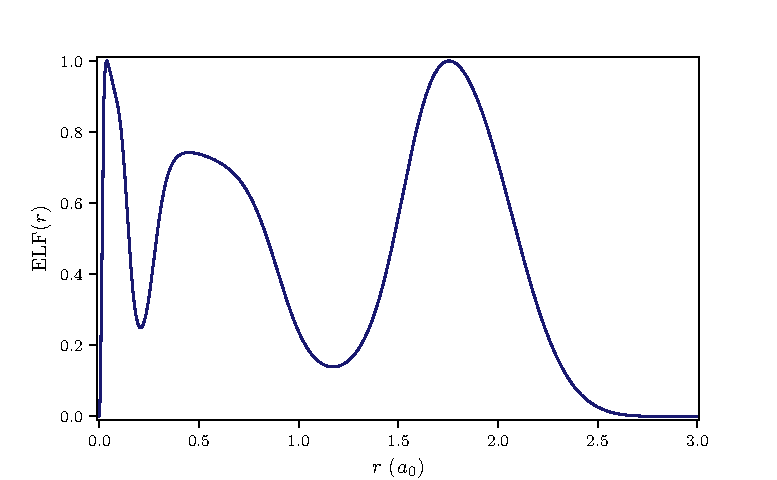
\includegraphics{figures/ELF_example.pdf} 
\label{Al:ELF_example} 
\caption{Electron localization function $\textrm{ELF}(r)$ for Aluminium at                     its solid density $\rho_\textrm{m}=2.7\ \textrm{g cm}^{-3}$ and                     temperature $T = 0.01\ \textrm{eV}$, for the Dirichlet                     boundary condition.} 
\end{figure}    \end{center}
    { \hspace*{\fill} \\}
    
    The next stage is to use the ELF to compute the number of electrons in a
given shell. This is done by finding the positions of the minima of the
ELF, and integrating the density between them, as explained in the main
paper. In atoMEC, we can access this data from the \texttt{N\_shell}
property of the \texttt{ELFTools} object:

    \begin{tcolorbox}[breakable, size=fbox, boxrule=1pt, pad at break*=1mm,colback=cellbackground, colframe=cellborder]
\prompt{In}{incolor}{24}{\boxspacing}
\begin{Verbatim}[commandchars=\\\{\}]
\PY{c+c1}{\PYZsh{} extract the number of electrons per shell}
\PY{n}{N\PYZus{}s} \PY{o}{=} \PY{n}{ELF\PYZus{}Al}\PY{o}{.}\PY{n}{N\PYZus{}shell}\PY{p}{[}\PY{l+m+mi}{0}\PY{p}{]}

\PY{k}{for} \PY{n}{i} \PY{o+ow}{in} \PY{n+nb}{range}\PY{p}{(}\PY{n+nb}{len}\PY{p}{(}\PY{n}{N\PYZus{}s}\PY{p}{)}\PY{p}{)}\PY{p}{:}
    \PY{n+nb}{print}\PY{p}{(}\PY{l+s+s2}{\PYZdq{}}\PY{l+s+s2}{The number of electrons in the n =}\PY{l+s+s2}{\PYZdq{}}\PY{p}{,} \PY{n}{i} \PY{o}{+} \PY{l+m+mi}{1}\PY{p}{,} \PY{l+s+s2}{\PYZdq{}}\PY{l+s+s2}{shell =}\PY{l+s+s2}{\PYZdq{}}\PY{p}{,} \PY{n+nb}{round}\PY{p}{(}\PY{n}{N\PYZus{}s}\PY{p}{[}\PY{n}{i}\PY{p}{]}\PY{p}{,} \PY{l+m+mi}{2}\PY{p}{)}\PY{p}{)}
\end{Verbatim}
\end{tcolorbox}

    \begin{Verbatim}[commandchars=\\\{\}]
The number of electrons in the n = 1 shell = 2.13
The number of electrons in the n = 2 shell = 7.72
The number of electrons in the n = 3 shell = 3.11
    \end{Verbatim}

    These numbers approximately match up to what we expect from ambient
Aluminium: 2 electrons in the \(n=1\) shell, 8 in the \(n=2\) shell, and
the remaining 3 electrons in the conduction band (which we call the
\(n=3\) shell here). As discussed in the main paper, extracting the MIS
from this output requires some user input based on physical intuition,
to decide which shells should be counted as bound and which free.

    \hypertarget{calculation-of-the-mis-using-the-kubogreenwood-formula}{%
\subsection{Calculation of the MIS using the Kubo--Greenwood
formula}\label{calculation-of-the-mis-using-the-kubogreenwood-formula}}

As seen in eq. (2) of the main text, the KG conductivity formula in a
finite system is given by

\begin{equation}
\sigma_{S_1,S_2} (\omega)= \frac{2\pi}{3V\omega} \sum_{i\in S_1} \sum_{j\in S_2} (f_i - f_j) |\langle \phi_i | \nabla | \phi_j \rangle|^2 \delta (\epsilon_j - \epsilon_i - \omega)\,,
\end{equation}

for subsets \(\{S_1\},\{S_2\}\) of the orbitals. In the spherically
symmetric case, this becomes

\begin{equation}
\sigma_{S_1,S_2}(\omega) = \frac{2\pi}{3V\omega} \sum_{nlm\in S_1} \sum_{n'l'm'\in S_2} (f_{nlm} - f_{n'l'm'}) |\langle \phi_{nlm} | \nabla | \phi_{n'l'm'} \rangle|^2 \delta (\epsilon_{n'l'm'} - \epsilon_{nlm} - \omega)\,.
\end{equation}

Note that, in the band-structure model, this becomes

\begin{equation}
\sigma_{S_1,S_2} (\omega) = \frac{2\pi}{3V\omega} \sum_k w_k \sum_{nlm\in S_1} \sum_{n'l'm'\in S_2} (f_{knlm} - f_{kn'l'm'}) |\langle \phi_{knlm} | \nabla | \phi_{kn'l'm'} \rangle|^2 \delta (\epsilon_{kn'l'm'} - \epsilon_{knlm} - \omega)\,,
\end{equation}

similar to the KG conductivity in plane-wave DFT codes. For simplicity,
and because in the end we shall only the KG conductivity with the
Dirichlet boundary condition, we shall present the equations without the
\(k\)-index. Since the summation only involves orbitals with the same
\(k\)-value, it is straightforward to re-introduce this at the end of
the derivation.

We focus first on the integral component of the equation for
\(\sigma(\omega)\), which is given by

\begin{align}
|\langle \phi_{knlm} | \nabla | \phi_{kn'l'm'} \rangle|^2 &= \sum_{i=1}^3 \langle \phi_{knlm} | \nabla_i | \phi_{kn'l'm'} \rangle \langle \phi_{kn'l'm'} | \nabla_i | \phi_{knlm} \rangle \\
&=3 \langle \phi_{knlm} | \nabla_z | \phi_{kn'l'm'} \rangle \langle \phi_{kn'l'm'} | \nabla_z | \phi_{knlm} \rangle\,,
\end{align}

where the second equation follows because the contribution from each
cartesian component of the gradient is identical in spherically
symmetric systems. We choose the \(z\) component because, in the
traditional transformation between cartesian and spherical co-ordinates,
this leads to a simpler set of equations. Let us now focus on the
following term,

\begin{align}
\langle \phi_{kn'l'm'} | \nabla_z | \phi_{knlm} \rangle&= \nabla_{nn'll'mm'}^z \\
&=R^{(d)}_{nn'll'} P^{(2)}_{lml'm'} \delta_{mm'} + R_{nn'll'} P^{(4)}_{lml'm'} \delta_{mm'},
\end{align}

which has been taken from this Ref. \onlinecite{Trickey_Kubo_Greenwood}.
We do not derive the above expression, but instead direct readers to the
aforementioned paper where it is derived in full. The terms in the above
expression are given by

\begin{align}
R^{(d)}_{nn'll'} &= 4\pi\int_0^{R_\textrm{VS}} \textrm{d}r r^2 X_{n'l'}(r) \frac{\textrm{d}X_{nl}(r)}{\textrm{d}r}\\
 R_{nn'll'} &= 4\pi\int_0^{R_\textrm{VS}} \textrm{d}r r X_{n'l'}(r) X_{nl}(r) \\
 P^{(2)}_{lml'm'} &= 2\pi C_{lm}C_{l'm'} \int_{-1}^{1} \textrm{d}x x P_{l'}^{m'} (x) P_{l}^{m}(x) \\
 P^{(4)}_{lml'm'} &= -2\pi C_{lm}C_{l'm'} \int_{-1}^{1} \textrm{d}x (1-x^2) P_{l'}^{m'} (x) \frac{\textrm{d}P_l^m(x)}{\textrm{d}x}\\
 C_{lm} &= \sqrt{\frac{2l+1}{4\pi}}\sqrt{\frac{(l-|m|)!}{(l+|m|)!)}}\,,
\end{align}

where \(P_l^m(x)\) are the Legendre polynomials. Note there are some
additional factors of \(4\pi\) in the above expressions compared to Ref.
\onlinecite{Trickey_Kubo_Greenwood}, due to different conventions in
normalization of the orbitals. Returning to the expression for
\(\sigma(\omega)\), we now have

\begin{equation}
\sigma_{S_1,S_2}(\omega) = \frac{2\pi}{V\omega} \sum_{nl\in S_1} \sum_{n'l'\in S_2} \sum_{m\in \{S1,S2\}} (f_{nl} - f_{n'l'}) |\nabla_{nn'll'm}^z|^2 \delta (\epsilon_{n'l'} - \epsilon_{nl} - \omega) \delta(l\pm 1 - l')\,.
\end{equation}

In the above, the double summation over \(m\) has been reduced to a
single summation because of the presence of the the \(\delta_{mm'}\) in
\(\nabla_{nn'll'mm'}^z\). Additionally, the \(\delta(l\pm 1 - l')\)
comes from sum rules in the evaluation of the \(P^{(2,4)}\) integrals.

Now, noting the relationship between the conductivity and the number of
electrons \(Z_{S1,S2}\) which contribute to that part of the
conductivity,

\begin{equation}
Z_{S1,S2} = \frac{2V}{\pi} \int_0^\infty \textrm{d}\omega \sigma_{S1,S2}(\omega)\,, 
\end{equation}

we substitute our AA conductivity formula into the above expression to
obtain

\begin{equation}
Z_{S1,S2} = 4 \sum_{nl\in S_1} \sum_{n'l'\in S_2} \sum_{m\in \{S1,S2\}} \frac{f_{nl} - f_{n'l'}}{\epsilon_{n'l'}-\epsilon_{nl}}|\nabla_{nn'll'm}^z|^2 \delta(l\pm 1 - l') \Theta (\epsilon_{n'l'}-\epsilon_{nl})
\end{equation}

In a conventional AA model, unlike in plane-wave DFT calculations, there
is no concept of a band-structure, which is problematic for determining
which subset of orbitals belong to the conducting vs valence bands. One
option could be to use the chemical potential \(\mu\) as a dividing
line, and define the valence orbitals as those below the chemical
potential, and the conduction orbitals as those above it. However, since
we have the band-structure AA model at our disposal, we can use that to
guide which orbitals belong in the conduction and valence bands. This is
just done manually (e.g.~by inspecting the DOS). We use this method even
for evaluating the KG conductivity with the Dirichlet boundary
condition.

In atoMEC the Kubo--Greenwood functionality is accessed through the
\texttt{kubo\_greenwood} module. We show how to extract the total number
of electrons (to check the sum rule is satisfied) and the number of free
electrons (i.e.~the MIS) below.

    \begin{tcolorbox}[breakable, size=fbox, boxrule=1pt, pad at break*=1mm,colback=cellbackground, colframe=cellborder]
\prompt{In}{incolor}{25}{\boxspacing}
\begin{Verbatim}[commandchars=\\\{\}]
\PY{c+c1}{\PYZsh{} first we re\PYZhy{}run the Al calculation with more unoccupied orbitals}
\PY{c+c1}{\PYZsh{} this is required because the KG method needs empty orbitals to converge}

\PY{c+c1}{\PYZsh{} set the values of nmax and lmax}
\PY{n}{nmax} \PY{o}{=} \PY{l+m+mi}{25}
\PY{n}{lmax} \PY{o}{=} \PY{l+m+mi}{10}

\PY{c+c1}{\PYZsh{} run the SCF calculation}
\PY{n}{output} \PY{o}{=} \PY{n}{Al\PYZus{}model}\PY{o}{.}\PY{n}{CalcEnergy}\PY{p}{(}
    \PY{n}{nmax}\PY{p}{,}
    \PY{n}{lmax}\PY{p}{,}
    \PY{n}{scf\PYZus{}params}\PY{o}{=}\PY{p}{\PYZob{}}\PY{l+s+s2}{\PYZdq{}}\PY{l+s+s2}{mixfrac}\PY{l+s+s2}{\PYZdq{}}\PY{p}{:} \PY{l+m+mf}{0.6}\PY{p}{,} \PY{l+s+s2}{\PYZdq{}}\PY{l+s+s2}{maxscf}\PY{l+s+s2}{\PYZdq{}}\PY{p}{:} \PY{l+m+mi}{50}\PY{p}{\PYZcb{}}\PY{p}{,}
    \PY{n}{grid\PYZus{}params}\PY{o}{=}\PY{p}{\PYZob{}}\PY{l+s+s2}{\PYZdq{}}\PY{l+s+s2}{ngrid}\PY{l+s+s2}{\PYZdq{}}\PY{p}{:} \PY{l+m+mi}{2000}\PY{p}{\PYZcb{}}\PY{p}{,}
    \PY{n}{write\PYZus{}info}\PY{o}{=}\PY{k+kc}{False}\PY{p}{,}
\PY{p}{)}
\end{Verbatim}
\end{tcolorbox}

    \begin{Verbatim}[commandchars=\\\{\}]
func:'CalcEnergy' took: 89.8896 sec
    \end{Verbatim}

    \begin{tcolorbox}[breakable, size=fbox, boxrule=1pt, pad at break*=1mm,colback=cellbackground, colframe=cellborder]
\prompt{In}{incolor}{26}{\boxspacing}
\begin{Verbatim}[commandchars=\\\{\}]
\PY{c+c1}{\PYZsh{} we need to define the \PYZsq{}valence\PYZsq{} orbitals, which actually means everything not in the conduction band}
\PY{c+c1}{\PYZsh{} for solid Al at room temperature the valence orbitals are 1s, 2s and 2p}
\PY{n}{valence\PYZus{}orbs} \PY{o}{=} \PY{p}{[}\PY{p}{(}\PY{l+m+mi}{0}\PY{p}{,} \PY{l+m+mi}{0}\PY{p}{)}\PY{p}{,} \PY{p}{(}\PY{l+m+mi}{1}\PY{p}{,} \PY{l+m+mi}{0}\PY{p}{)}\PY{p}{,} \PY{p}{(}\PY{l+m+mi}{0}\PY{p}{,} \PY{l+m+mi}{1}\PY{p}{)}\PY{p}{]}

\PY{c+c1}{\PYZsh{} set up the Kubo\PYZhy{}Greenwood object}
\PY{n}{kg} \PY{o}{=} \PY{n}{localization}\PY{o}{.}\PY{n}{KuboGreenwood}\PY{p}{(}\PY{n}{output}\PY{p}{[}\PY{l+s+s2}{\PYZdq{}}\PY{l+s+s2}{orbitals}\PY{l+s+s2}{\PYZdq{}}\PY{p}{]}\PY{p}{,} \PY{n}{valence\PYZus{}orbs}\PY{o}{=}\PY{n}{valence\PYZus{}orbs}\PY{p}{)}

\PY{c+c1}{\PYZsh{} compute the total number of electrons}
\PY{n}{N\PYZus{}tot} \PY{o}{=} \PY{n}{kg}\PY{o}{.}\PY{n}{N\PYZus{}tot}

\PY{c+c1}{\PYZsh{} compute the number of free electrons}
\PY{n}{N\PYZus{}free} \PY{o}{=} \PY{n}{kg}\PY{o}{.}\PY{n}{N\PYZus{}free}

\PY{c+c1}{\PYZsh{} print the output}
\PY{n+nb}{print}\PY{p}{(}\PY{l+s+s2}{\PYZdq{}}\PY{l+s+s2}{Total number of electrons = }\PY{l+s+s2}{\PYZdq{}}\PY{p}{,} \PY{n+nb}{round}\PY{p}{(}\PY{n}{N\PYZus{}tot}\PY{p}{,} \PY{l+m+mi}{2}\PY{p}{)}\PY{p}{)}
\PY{n+nb}{print}\PY{p}{(}\PY{l+s+s2}{\PYZdq{}}\PY{l+s+s2}{Number of free electrons = }\PY{l+s+s2}{\PYZdq{}}\PY{p}{,} \PY{n+nb}{round}\PY{p}{(}\PY{n}{N\PYZus{}free}\PY{p}{,} \PY{l+m+mi}{2}\PY{p}{)}\PY{p}{)}
\end{Verbatim}
\end{tcolorbox}

    \begin{Verbatim}[commandchars=\\\{\}]
Total number of electrons =  12.95
Number of free electrons =  3.29
    \end{Verbatim}

    In the above example, it can be seen that the total number of electrons
equals 12.95, which is very close to the expected value of 13 for
Alunimium (less than 1\% difference). Therefore it seems the values of
\texttt{nmax} and \texttt{lmax} are large enough for the KG calculation
to be converged. The number of free electrons is 3.29, which is close to
the value of 3 that might be expected from physical intuition.

    \hypertarget{results}{%
\section{Results}\label{results}}

The inputs to reproduce the results in the main paper will be made
available upon publication.

    \begin{tcolorbox}[breakable, size=fbox, boxrule=1pt, pad at break*=1mm,colback=cellbackground, colframe=cellborder]
\prompt{In}{incolor}{ }{\boxspacing}
\begin{Verbatim}[commandchars=\\\{\}]

\end{Verbatim}
\end{tcolorbox}

    \hypertarget{results}{%
\section{Results}\label{results}}

In this section, we run through the calculations presented in the paper.
In the first sub-section, we run the SCF calculations to get the KS
orbitals and density. These are used as inputs for computing the MIS via
the different methods, which we run through in the following
sub-section. Note that the primary objective of atoMEC is not
computationally efficiency, and thus the each SCF calculation may take
up to \textasciitilde{}20 minutes for the inputs used in the paper. If
you wish to run all the SCF calculations, we provide all necessary
inputs but we suggest to run the calculations on a separate cluster.

Alternatively, feel free to skip the SCF sub-section and proceed
directly to the post-SCF analysis. All the data required for this
subsequent step is already provided.

\hypertarget{scf-calculations-carbon}{%
\subsection{SCF calculations: Carbon}\label{scf-calculations-carbon}}

In you wish to run the SCF calculations, please set
\texttt{run\_SCF\_calcs\ =\ True} below:

    \begin{tcolorbox}[breakable, size=fbox, boxrule=1pt, pad at break*=1mm,colback=cellbackground, colframe=cellborder]
\prompt{In}{incolor}{ }{\boxspacing}
\begin{Verbatim}[commandchars=\\\{\}]
\PY{c+c1}{\PYZsh{} whether to run the SCF calculations}
\PY{n}{run\PYZus{}SCF\PYZus{}calcs} \PY{o}{=} \PY{k+kc}{True}
\end{Verbatim}
\end{tcolorbox}

    First, we set up the calculations for Carbon at \(T=100\) eV, under a
range of densities.

    \begin{tcolorbox}[breakable, size=fbox, boxrule=1pt, pad at break*=1mm,colback=cellbackground, colframe=cellborder]
\prompt{In}{incolor}{ }{\boxspacing}
\begin{Verbatim}[commandchars=\\\{\}]
\PY{k+kn}{import} \PY{n+nn}{pickle} \PY{k}{as} \PY{n+nn}{pkl}

\PY{c+c1}{\PYZsh{} ensure parallelism is on}
\PY{n}{config}\PY{o}{.}\PY{n}{numcores} \PY{o}{=} \PY{l+m+mi}{9}
\PY{c+c1}{\PYZsh{} set up the base Carbon atom}
\PY{n}{C\PYZus{}atom} \PY{o}{=} \PY{n}{Atom}\PY{p}{(}\PY{l+s+s2}{\PYZdq{}}\PY{l+s+s2}{C}\PY{l+s+s2}{\PYZdq{}}\PY{p}{,} \PY{l+m+mi}{100}\PY{p}{,} \PY{n}{density}\PY{o}{=}\PY{l+m+mf}{1.0}\PY{p}{,} \PY{n}{units\PYZus{}temp}\PY{o}{=}\PY{l+s+s2}{\PYZdq{}}\PY{l+s+s2}{eV}\PY{l+s+s2}{\PYZdq{}}\PY{p}{,} \PY{n}{write\PYZus{}info}\PY{o}{=}\PY{k+kc}{False}\PY{p}{)}
\PY{c+c1}{\PYZsh{} set up the base model}
\PY{n}{model} \PY{o}{=} \PY{n}{models}\PY{o}{.}\PY{n}{ISModel}\PY{p}{(}\PY{n}{C\PYZus{}atom}\PY{p}{,} \PY{n}{unbound}\PY{o}{=}\PY{l+s+s2}{\PYZdq{}}\PY{l+s+s2}{quantum}\PY{l+s+s2}{\PYZdq{}}\PY{p}{,} \PY{n}{write\PYZus{}info}\PY{o}{=}\PY{k+kc}{False}\PY{p}{)}
\PY{c+c1}{\PYZsh{} define the boundary conditions}
\PY{n}{bcs} \PY{o}{=} \PY{p}{[}\PY{l+s+s2}{\PYZdq{}}\PY{l+s+s2}{dirichlet}\PY{l+s+s2}{\PYZdq{}}\PY{p}{,} \PY{l+s+s2}{\PYZdq{}}\PY{l+s+s2}{neumann}\PY{l+s+s2}{\PYZdq{}}\PY{p}{,} \PY{l+s+s2}{\PYZdq{}}\PY{l+s+s2}{bands}\PY{l+s+s2}{\PYZdq{}}\PY{p}{]}
\PY{c+c1}{\PYZsh{} define the densities}
\PY{n}{densities} \PY{o}{=} \PY{n}{np}\PY{o}{.}\PY{n}{array}\PY{p}{(}\PY{p}{[}\PY{l+m+mi}{1}\PY{p}{,} \PY{l+m+mi}{2}\PY{p}{,} \PY{l+m+mi}{5}\PY{p}{,} \PY{l+m+mi}{10}\PY{p}{,} \PY{l+m+mi}{20}\PY{p}{,} \PY{l+m+mi}{50}\PY{p}{,} \PY{l+m+mi}{80}\PY{p}{,} \PY{l+m+mi}{100}\PY{p}{,} \PY{l+m+mi}{150}\PY{p}{,} \PY{l+m+mi}{200}\PY{p}{,} \PY{l+m+mi}{300}\PY{p}{,} \PY{l+m+mi}{400}\PY{p}{]}\PY{p}{,} \PY{n}{dtype}\PY{o}{=}\PY{n+nb}{float}\PY{p}{)}
\PY{c+c1}{\PYZsh{} set the lmax parameter (same for all bcs)}
\PY{n}{lmax} \PY{o}{=} \PY{l+m+mi}{20}
\PY{c+c1}{\PYZsh{} grid parameters}
\PY{n}{grid\PYZus{}params} \PY{o}{=} \PY{p}{\PYZob{}}\PY{l+s+s2}{\PYZdq{}}\PY{l+s+s2}{ngrid}\PY{l+s+s2}{\PYZdq{}}\PY{p}{:} \PY{l+m+mi}{1500}\PY{p}{\PYZcb{}}
\PY{c+c1}{\PYZsh{} band\PYZus{}parameters}
\PY{n}{band\PYZus{}params} \PY{o}{=} \PY{p}{\PYZob{}}\PY{l+s+s2}{\PYZdq{}}\PY{l+s+s2}{nkpts}\PY{l+s+s2}{\PYZdq{}}\PY{p}{:} \PY{l+m+mi}{50}\PY{p}{\PYZcb{}}
\PY{c+c1}{\PYZsh{} base directory}
\PY{n}{basedir} \PY{o}{=} \PY{l+s+s2}{\PYZdq{}}\PY{l+s+s2}{/home/callow46/mean\PYZus{}ionization\PYZus{}paper}\PY{l+s+s2}{\PYZdq{}}

\PY{k}{if} \PY{n}{run\PYZus{}SCF\PYZus{}calcs}\PY{p}{:}
    \PY{c+c1}{\PYZsh{} loop over boundary conditions}
    \PY{k}{for} \PY{n}{bc} \PY{o+ow}{in} \PY{n}{bcs}\PY{p}{:}
        \PY{c+c1}{\PYZsh{} change into the bc directory}
        \PY{n}{os}\PY{o}{.}\PY{n}{chdir}\PY{p}{(}\PY{n}{basedir} \PY{o}{+} \PY{l+s+s2}{\PYZdq{}}\PY{l+s+s2}{/results/Carbon/}\PY{l+s+s2}{\PYZdq{}} \PY{o}{+} \PY{n}{bc} \PY{o}{+} \PY{l+s+s2}{\PYZdq{}}\PY{l+s+s2}{/}\PY{l+s+s2}{\PYZdq{}}\PY{p}{)}
        \PY{c+c1}{\PYZsh{} set the boundary condition}
        \PY{n}{model}\PY{o}{.}\PY{n}{bc} \PY{o}{=} \PY{n}{bc}
        \PY{c+c1}{\PYZsh{} dirichlet needs more eigenvalues since empty states required for Kubo\PYZhy{}Greenwood}
        \PY{k}{if} \PY{n}{bc} \PY{o}{==} \PY{l+s+s2}{\PYZdq{}}\PY{l+s+s2}{dirichlet}\PY{l+s+s2}{\PYZdq{}}\PY{p}{:}
            \PY{n}{nmax} \PY{o}{=} \PY{l+m+mi}{30}
        \PY{k}{else}\PY{p}{:}
            \PY{n}{nmax} \PY{o}{=} \PY{l+m+mi}{20}
        \PY{c+c1}{\PYZsh{} loop over the densities}
        \PY{k}{for} \PY{n}{density} \PY{o+ow}{in} \PY{n}{densities}\PY{p}{:}
            \PY{c+c1}{\PYZsh{} set the output to an external file}
            \PY{n}{sys}\PY{o}{.}\PY{n}{stdout} \PY{o}{=} \PY{n+nb}{open}\PY{p}{(}\PY{l+s+s2}{\PYZdq{}}\PY{l+s+s2}{C\PYZus{}}\PY{l+s+s2}{\PYZdq{}} \PY{o}{+} \PY{n+nb}{str}\PY{p}{(}\PY{n}{density}\PY{p}{)} \PY{o}{+} \PY{l+s+s2}{\PYZdq{}}\PY{l+s+s2}{.log}\PY{l+s+s2}{\PYZdq{}}\PY{p}{,} \PY{l+s+s2}{\PYZdq{}}\PY{l+s+s2}{w}\PY{l+s+s2}{\PYZdq{}}\PY{p}{)}
            \PY{c+c1}{\PYZsh{} set the density}
            \PY{n}{C\PYZus{}atom}\PY{o}{.}\PY{n}{density} \PY{o}{=} \PY{n}{density}
            \PY{c+c1}{\PYZsh{} run the SCF calculation}
            \PY{n}{output} \PY{o}{=} \PY{n}{model}\PY{o}{.}\PY{n}{CalcEnergy}\PY{p}{(}
                \PY{n}{nmax}\PY{p}{,}
                \PY{n}{lmax}\PY{p}{,}
                \PY{n}{grid\PYZus{}params}\PY{o}{=}\PY{n}{grid\PYZus{}params}\PY{p}{,}
                \PY{n}{band\PYZus{}params}\PY{o}{=}\PY{n}{band\PYZus{}params}\PY{p}{,}
                \PY{n}{dos\PYZus{}file}\PY{o}{=}\PY{l+s+s2}{\PYZdq{}}\PY{l+s+s2}{dos\PYZus{}}\PY{l+s+s2}{\PYZdq{}} \PY{o}{+} \PY{n+nb}{str}\PY{p}{(}\PY{n}{density}\PY{p}{)} \PY{o}{+} \PY{l+s+s2}{\PYZdq{}}\PY{l+s+s2}{.csv}\PY{l+s+s2}{\PYZdq{}}\PY{p}{,}
            \PY{p}{)}
            \PY{c+c1}{\PYZsh{} save the orbitals and density output}
            \PY{n}{orbfile} \PY{o}{=} \PY{l+s+s2}{\PYZdq{}}\PY{l+s+s2}{C\PYZus{}orbs\PYZus{}}\PY{l+s+s2}{\PYZdq{}} \PY{o}{+} \PY{n+nb}{str}\PY{p}{(}\PY{n}{density}\PY{p}{)} \PY{o}{+} \PY{l+s+s2}{\PYZdq{}}\PY{l+s+s2}{.pkl}\PY{l+s+s2}{\PYZdq{}}
            \PY{n}{densfile} \PY{o}{=} \PY{l+s+s2}{\PYZdq{}}\PY{l+s+s2}{C\PYZus{}dens\PYZus{}}\PY{l+s+s2}{\PYZdq{}} \PY{o}{+} \PY{n+nb}{str}\PY{p}{(}\PY{n}{density}\PY{p}{)} \PY{o}{+} \PY{l+s+s2}{\PYZdq{}}\PY{l+s+s2}{.pkl}\PY{l+s+s2}{\PYZdq{}}
            \PY{k}{with} \PY{n+nb}{open}\PY{p}{(}\PY{n}{orbfile}\PY{p}{,} \PY{l+s+s2}{\PYZdq{}}\PY{l+s+s2}{wb}\PY{l+s+s2}{\PYZdq{}}\PY{p}{)} \PY{k}{as} \PY{n}{f}\PY{p}{:}
                \PY{n}{pkl}\PY{o}{.}\PY{n}{dump}\PY{p}{(}\PY{n}{output}\PY{p}{[}\PY{l+s+s2}{\PYZdq{}}\PY{l+s+s2}{orbitals}\PY{l+s+s2}{\PYZdq{}}\PY{p}{]}\PY{p}{,} \PY{n}{f}\PY{p}{)}
            \PY{k}{with} \PY{n+nb}{open}\PY{p}{(}\PY{n}{densfile}\PY{p}{,} \PY{l+s+s2}{\PYZdq{}}\PY{l+s+s2}{wb}\PY{l+s+s2}{\PYZdq{}}\PY{p}{)} \PY{k}{as} \PY{n}{f}\PY{p}{:}
                \PY{n}{pkl}\PY{o}{.}\PY{n}{dump}\PY{p}{(}\PY{n}{output}\PY{p}{[}\PY{l+s+s2}{\PYZdq{}}\PY{l+s+s2}{density}\PY{l+s+s2}{\PYZdq{}}\PY{p}{]}\PY{p}{,} \PY{n}{f}\PY{p}{)}
                
\PY{c+c1}{\PYZsh{} reset output to terminal}
\PY{n}{sys}\PY{o}{.}\PY{n}{stdout} \PY{o}{=} \PY{n}{default\PYZus{}stdout}
\end{Verbatim}
\end{tcolorbox}

    \hypertarget{scf-calculations-beryllium}{%
\subsection{SCF calculations:
Beryllium}\label{scf-calculations-beryllium}}

Next, we set up the calculations for Beryllium with fixed density
\(\rho_\textrm{m} = 1.85\ \textrm{g cm}^{-3}\), for a range of
temperatures.

    \begin{tcolorbox}[breakable, size=fbox, boxrule=1pt, pad at break*=1mm,colback=cellbackground, colframe=cellborder]
\prompt{In}{incolor}{ }{\boxspacing}
\begin{Verbatim}[commandchars=\\\{\}]
\PY{c+c1}{\PYZsh{} set up the base Beryllium atom}
\PY{n}{Be\PYZus{}atom} \PY{o}{=} \PY{n}{Atom}\PY{p}{(}\PY{l+s+s2}{\PYZdq{}}\PY{l+s+s2}{Be}\PY{l+s+s2}{\PYZdq{}}\PY{p}{,} \PY{l+m+mi}{1}\PY{p}{,} \PY{n}{density}\PY{o}{=}\PY{l+m+mf}{1.85}\PY{p}{,} \PY{n}{units\PYZus{}temp}\PY{o}{=}\PY{l+s+s2}{\PYZdq{}}\PY{l+s+s2}{eV}\PY{l+s+s2}{\PYZdq{}}\PY{p}{,} \PY{n}{write\PYZus{}info}\PY{o}{=}\PY{k+kc}{False}\PY{p}{)}
\PY{c+c1}{\PYZsh{} set up the base model}
\PY{n}{model} \PY{o}{=} \PY{n}{models}\PY{o}{.}\PY{n}{ISModel}\PY{p}{(}\PY{n}{Be\PYZus{}atom}\PY{p}{,} \PY{n}{unbound}\PY{o}{=}\PY{l+s+s2}{\PYZdq{}}\PY{l+s+s2}{quantum}\PY{l+s+s2}{\PYZdq{}}\PY{p}{,} \PY{n}{write\PYZus{}info}\PY{o}{=}\PY{k+kc}{False}\PY{p}{)}
\PY{c+c1}{\PYZsh{} define the temperatures}
\PY{n}{temps} \PY{o}{=} \PY{n}{np}\PY{o}{.}\PY{n}{arange}\PY{p}{(}\PY{l+m+mi}{2}\PY{p}{,} \PY{l+m+mi}{86}\PY{p}{,} \PY{l+m+mi}{4}\PY{p}{,} \PY{n}{dtype}\PY{o}{=}\PY{n+nb}{float}\PY{p}{)}
\PY{c+c1}{\PYZsh{} set the lmax parameter (same for all bcs)}
\PY{n}{lmax} \PY{o}{=} \PY{l+m+mi}{15}
\PY{c+c1}{\PYZsh{} grid parameters}
\PY{n}{grid\PYZus{}params} \PY{o}{=} \PY{p}{\PYZob{}}\PY{l+s+s2}{\PYZdq{}}\PY{l+s+s2}{ngrid}\PY{l+s+s2}{\PYZdq{}}\PY{p}{:} \PY{l+m+mi}{1500}\PY{p}{\PYZcb{}}

\PY{k}{if} \PY{n}{run\PYZus{}SCF\PYZus{}calcs}\PY{p}{:}
    \PY{c+c1}{\PYZsh{} loop over boundary conditions}
    \PY{k}{for} \PY{n}{bc} \PY{o+ow}{in} \PY{n}{bcs}\PY{p}{:}
        \PY{c+c1}{\PYZsh{} change into the bc directory}
        \PY{n}{os}\PY{o}{.}\PY{n}{chdir}\PY{p}{(}\PY{n}{basedir} \PY{o}{+} \PY{l+s+s2}{\PYZdq{}}\PY{l+s+s2}{/results/Beryllium/}\PY{l+s+s2}{\PYZdq{}} \PY{o}{+} \PY{n}{bc} \PY{o}{+} \PY{l+s+s2}{\PYZdq{}}\PY{l+s+s2}{/}\PY{l+s+s2}{\PYZdq{}}\PY{p}{)}
        \PY{c+c1}{\PYZsh{} set the boundary condition}
        \PY{n}{model}\PY{o}{.}\PY{n}{bc} \PY{o}{=} \PY{n}{bc}
        \PY{c+c1}{\PYZsh{} dirichlet needs more eigenvalues since empty states required for Kubo\PYZhy{}Greenwood}
        \PY{k}{if} \PY{n}{bc} \PY{o}{==} \PY{l+s+s2}{\PYZdq{}}\PY{l+s+s2}{dirichlet}\PY{l+s+s2}{\PYZdq{}}\PY{p}{:}
            \PY{n}{nmax} \PY{o}{=} \PY{l+m+mi}{30}
        \PY{k}{else}\PY{p}{:}
            \PY{n}{nmax} \PY{o}{=} \PY{l+m+mi}{15}
        \PY{k}{if} \PY{n}{bc} \PY{o}{==} \PY{l+s+s2}{\PYZdq{}}\PY{l+s+s2}{bands}\PY{l+s+s2}{\PYZdq{}}\PY{p}{:}
            \PY{n}{nkpts} \PY{o}{=} \PY{l+m+mi}{50}
        \PY{k}{else}\PY{p}{:}
            \PY{n}{nkpts} \PY{o}{=} \PY{l+m+mi}{1}
        \PY{c+c1}{\PYZsh{} loop over the densities}
        \PY{k}{for} \PY{n}{temp} \PY{o+ow}{in} \PY{n}{temps}\PY{p}{:}
            \PY{c+c1}{\PYZsh{} set the output to an external file}
            \PY{n}{sys}\PY{o}{.}\PY{n}{stdout} \PY{o}{=} \PY{n+nb}{open}\PY{p}{(}\PY{l+s+s2}{\PYZdq{}}\PY{l+s+s2}{Be\PYZus{}}\PY{l+s+s2}{\PYZdq{}} \PY{o}{+} \PY{n+nb}{str}\PY{p}{(}\PY{n}{temp}\PY{p}{)} \PY{o}{+} \PY{l+s+s2}{\PYZdq{}}\PY{l+s+s2}{.log}\PY{l+s+s2}{\PYZdq{}}\PY{p}{,} \PY{l+s+s2}{\PYZdq{}}\PY{l+s+s2}{w}\PY{l+s+s2}{\PYZdq{}}\PY{p}{)}
            \PY{c+c1}{\PYZsh{} set the density}
            \PY{n}{Be\PYZus{}atom}\PY{o}{.}\PY{n}{temp} \PY{o}{=} \PY{n}{temp}
            \PY{c+c1}{\PYZsh{} run the SCF calculation}
            \PY{n}{output} \PY{o}{=} \PY{n}{model}\PY{o}{.}\PY{n}{CalcEnergy}\PY{p}{(}
                \PY{n}{nmax}\PY{p}{,}
                \PY{n}{lmax}\PY{p}{,}
                \PY{n}{grid\PYZus{}params}\PY{o}{=}\PY{n}{grid\PYZus{}params}\PY{p}{,}
                \PY{n}{band\PYZus{}params}\PY{o}{=}\PY{p}{\PYZob{}}\PY{l+s+s2}{\PYZdq{}}\PY{l+s+s2}{nkpts}\PY{l+s+s2}{\PYZdq{}}\PY{p}{:} \PY{n}{nkpts}\PY{p}{\PYZcb{}}\PY{p}{,}
            \PY{p}{)}
            \PY{c+c1}{\PYZsh{} save the orbitals and density output}
            \PY{n}{orbfile} \PY{o}{=} \PY{l+s+s2}{\PYZdq{}}\PY{l+s+s2}{Be\PYZus{}orbs\PYZus{}}\PY{l+s+s2}{\PYZdq{}} \PY{o}{+} \PY{n+nb}{str}\PY{p}{(}\PY{n}{temp}\PY{p}{)} \PY{o}{+} \PY{l+s+s2}{\PYZdq{}}\PY{l+s+s2}{.pkl}\PY{l+s+s2}{\PYZdq{}}
            \PY{n}{densfile} \PY{o}{=} \PY{l+s+s2}{\PYZdq{}}\PY{l+s+s2}{Be\PYZus{}dens\PYZus{}}\PY{l+s+s2}{\PYZdq{}} \PY{o}{+} \PY{n+nb}{str}\PY{p}{(}\PY{n}{temp}\PY{p}{)} \PY{o}{+} \PY{l+s+s2}{\PYZdq{}}\PY{l+s+s2}{.pkl}\PY{l+s+s2}{\PYZdq{}}
            \PY{k}{with} \PY{n+nb}{open}\PY{p}{(}\PY{n}{orbfile}\PY{p}{,} \PY{l+s+s2}{\PYZdq{}}\PY{l+s+s2}{wb}\PY{l+s+s2}{\PYZdq{}}\PY{p}{)} \PY{k}{as} \PY{n}{f}\PY{p}{:}
                \PY{n}{pkl}\PY{o}{.}\PY{n}{dump}\PY{p}{(}\PY{n}{output}\PY{p}{[}\PY{l+s+s2}{\PYZdq{}}\PY{l+s+s2}{orbitals}\PY{l+s+s2}{\PYZdq{}}\PY{p}{]}\PY{p}{,} \PY{n}{f}\PY{p}{,} \PY{n}{protocol}\PY{o}{=}\PY{n}{pkl}\PY{o}{.}\PY{n}{HIGHEST\PYZus{}PROTOCOL}\PY{p}{)}
            \PY{k}{with} \PY{n+nb}{open}\PY{p}{(}\PY{n}{densfile}\PY{p}{,} \PY{l+s+s2}{\PYZdq{}}\PY{l+s+s2}{wb}\PY{l+s+s2}{\PYZdq{}}\PY{p}{)} \PY{k}{as} \PY{n}{f}\PY{p}{:}
                \PY{n}{pkl}\PY{o}{.}\PY{n}{dump}\PY{p}{(}\PY{n}{output}\PY{p}{[}\PY{l+s+s2}{\PYZdq{}}\PY{l+s+s2}{density}\PY{l+s+s2}{\PYZdq{}}\PY{p}{]}\PY{p}{,} \PY{n}{f}\PY{p}{,} \PY{n}{protocol}\PY{o}{=}\PY{n}{pkl}\PY{o}{.}\PY{n}{HIGHEST\PYZus{}PROTOCOL}\PY{p}{)}

\PY{c+c1}{\PYZsh{} reset output to terminal}
\PY{n}{sys}\PY{o}{.}\PY{n}{stdout} \PY{o}{=} \PY{n}{default\PYZus{}stdout}
\end{Verbatim}
\end{tcolorbox}

    \hypertarget{scf-calculations-aluminium-i}{%
\subsection{SCF calculations: Aluminium
(i)}\label{scf-calculations-aluminium-i}}

We first run the necessary SCF calculations for the first Aluminium
experiment, for which the density is fixed at \(2.7 \textrm{g cm}^{-3}\)
and the temperature is varied between 10 and 30 eV.

    \begin{tcolorbox}[breakable, size=fbox, boxrule=1pt, pad at break*=1mm,colback=cellbackground, colframe=cellborder]
\prompt{In}{incolor}{ }{\boxspacing}
\begin{Verbatim}[commandchars=\\\{\}]
\PY{c+c1}{\PYZsh{} set up the base Aluninium atom}
\PY{n}{Al\PYZus{}atom} \PY{o}{=} \PY{n}{Atom}\PY{p}{(}\PY{l+s+s2}{\PYZdq{}}\PY{l+s+s2}{Al}\PY{l+s+s2}{\PYZdq{}}\PY{p}{,} \PY{l+m+mi}{10}\PY{p}{,} \PY{n}{density}\PY{o}{=}\PY{l+m+mf}{2.7}\PY{p}{,} \PY{n}{units\PYZus{}temp}\PY{o}{=}\PY{l+s+s2}{\PYZdq{}}\PY{l+s+s2}{eV}\PY{l+s+s2}{\PYZdq{}}\PY{p}{,} \PY{n}{write\PYZus{}info}\PY{o}{=}\PY{k+kc}{False}\PY{p}{)}
\PY{c+c1}{\PYZsh{} set up the base model}
\PY{n}{model} \PY{o}{=} \PY{n}{models}\PY{o}{.}\PY{n}{ISModel}\PY{p}{(}\PY{n}{Al\PYZus{}atom}\PY{p}{,} \PY{n}{unbound}\PY{o}{=}\PY{l+s+s2}{\PYZdq{}}\PY{l+s+s2}{quantum}\PY{l+s+s2}{\PYZdq{}}\PY{p}{,} \PY{n}{write\PYZus{}info}\PY{o}{=}\PY{k+kc}{False}\PY{p}{)}
\PY{c+c1}{\PYZsh{} define the temperatures}
\PY{n}{temps} \PY{o}{=} \PY{n}{np}\PY{o}{.}\PY{n}{arange}\PY{p}{(}\PY{l+m+mi}{10}\PY{p}{,} \PY{l+m+mi}{36}\PY{p}{,} \PY{l+m+mi}{1}\PY{p}{,} \PY{n}{dtype}\PY{o}{=}\PY{n+nb}{float}\PY{p}{)}
\PY{c+c1}{\PYZsh{} grid parameters}
\PY{n}{grid\PYZus{}params} \PY{o}{=} \PY{p}{\PYZob{}}\PY{l+s+s2}{\PYZdq{}}\PY{l+s+s2}{ngrid}\PY{l+s+s2}{\PYZdq{}}\PY{p}{:} \PY{l+m+mi}{1500}\PY{p}{\PYZcb{}}

\PY{k}{if} \PY{n}{run\PYZus{}SCF\PYZus{}calcs}\PY{p}{:}
    \PY{c+c1}{\PYZsh{} loop over boundary conditions}
    \PY{k}{for} \PY{n}{bc} \PY{o+ow}{in} \PY{n}{bcs}\PY{p}{:}
        \PY{c+c1}{\PYZsh{} change into the bc directory}
        \PY{n}{os}\PY{o}{.}\PY{n}{chdir}\PY{p}{(}\PY{n}{basedir} \PY{o}{+} \PY{l+s+s2}{\PYZdq{}}\PY{l+s+s2}{/results/Aluminium/expt\PYZus{}comp\PYZus{}1}\PY{l+s+s2}{\PYZdq{}} \PY{o}{+} \PY{n}{bc} \PY{o}{+} \PY{l+s+s2}{\PYZdq{}}\PY{l+s+s2}{/}\PY{l+s+s2}{\PYZdq{}}\PY{p}{)}
        \PY{c+c1}{\PYZsh{} set the boundary condition}
        \PY{n}{model}\PY{o}{.}\PY{n}{bc} \PY{o}{=} \PY{n}{bc}
        \PY{c+c1}{\PYZsh{} dirichlet needs more eigenvalues since empty states required for Kubo\PYZhy{}Greenwood}
        \PY{k}{if} \PY{n}{bc} \PY{o}{==} \PY{l+s+s2}{\PYZdq{}}\PY{l+s+s2}{dirichlet}\PY{l+s+s2}{\PYZdq{}}\PY{p}{:}
            \PY{n}{nmax} \PY{o}{=} \PY{l+m+mi}{30}
            \PY{n}{lmax} \PY{o}{=} \PY{l+m+mi}{20}
        \PY{k}{else}\PY{p}{:}
            \PY{n}{nmax} \PY{o}{=} \PY{l+m+mi}{10}
            \PY{n}{lmax} \PY{o}{=} \PY{l+m+mi}{15}
        \PY{k}{if} \PY{n}{bc} \PY{o}{==} \PY{l+s+s2}{\PYZdq{}}\PY{l+s+s2}{bands}\PY{l+s+s2}{\PYZdq{}}\PY{p}{:}
            \PY{n}{nkpts} \PY{o}{=} \PY{l+m+mi}{50}
        \PY{k}{else}\PY{p}{:}
            \PY{n}{nkpts} \PY{o}{=} \PY{l+m+mi}{1}
        \PY{c+c1}{\PYZsh{} loop over the densities}
        \PY{k}{for} \PY{n}{temp} \PY{o+ow}{in} \PY{n}{temps}\PY{p}{:}
            \PY{c+c1}{\PYZsh{} set the output to an external file}
            \PY{n}{sys}\PY{o}{.}\PY{n}{stdout} \PY{o}{=} \PY{n+nb}{open}\PY{p}{(}\PY{l+s+s2}{\PYZdq{}}\PY{l+s+s2}{Al\PYZus{}}\PY{l+s+s2}{\PYZdq{}} \PY{o}{+} \PY{n+nb}{str}\PY{p}{(}\PY{n}{temp}\PY{p}{)} \PY{o}{+} \PY{l+s+s2}{\PYZdq{}}\PY{l+s+s2}{.log}\PY{l+s+s2}{\PYZdq{}}\PY{p}{,} \PY{l+s+s2}{\PYZdq{}}\PY{l+s+s2}{w}\PY{l+s+s2}{\PYZdq{}}\PY{p}{)}
            \PY{c+c1}{\PYZsh{} set the density}
            \PY{n}{Al\PYZus{}atom}\PY{o}{.}\PY{n}{temp} \PY{o}{=} \PY{n}{temp}
            \PY{c+c1}{\PYZsh{} run the SCF calculation}
            \PY{n}{output} \PY{o}{=} \PY{n}{model}\PY{o}{.}\PY{n}{CalcEnergy}\PY{p}{(}
                \PY{n}{nmax}\PY{p}{,}
                \PY{n}{lmax}\PY{p}{,}
                \PY{n}{grid\PYZus{}params}\PY{o}{=}\PY{n}{grid\PYZus{}params}\PY{p}{,}
                \PY{n}{band\PYZus{}params}\PY{o}{=}\PY{p}{\PYZob{}}\PY{l+s+s2}{\PYZdq{}}\PY{l+s+s2}{nkpts}\PY{l+s+s2}{\PYZdq{}}\PY{p}{:} \PY{n}{nkpts}\PY{p}{\PYZcb{}}\PY{p}{,}
            \PY{p}{)}
            \PY{c+c1}{\PYZsh{} save the orbitals and density output}
            \PY{n}{orbfile} \PY{o}{=} \PY{l+s+s2}{\PYZdq{}}\PY{l+s+s2}{Al\PYZus{}orbs\PYZus{}}\PY{l+s+s2}{\PYZdq{}} \PY{o}{+} \PY{n+nb}{str}\PY{p}{(}\PY{n}{temp}\PY{p}{)} \PY{o}{+} \PY{l+s+s2}{\PYZdq{}}\PY{l+s+s2}{.pkl}\PY{l+s+s2}{\PYZdq{}}
            \PY{n}{densfile} \PY{o}{=} \PY{l+s+s2}{\PYZdq{}}\PY{l+s+s2}{Al\PYZus{}dens\PYZus{}}\PY{l+s+s2}{\PYZdq{}} \PY{o}{+} \PY{n+nb}{str}\PY{p}{(}\PY{n}{temp}\PY{p}{)} \PY{o}{+} \PY{l+s+s2}{\PYZdq{}}\PY{l+s+s2}{.pkl}\PY{l+s+s2}{\PYZdq{}}
            \PY{k}{with} \PY{n+nb}{open}\PY{p}{(}\PY{n}{orbfile}\PY{p}{,} \PY{l+s+s2}{\PYZdq{}}\PY{l+s+s2}{wb}\PY{l+s+s2}{\PYZdq{}}\PY{p}{)} \PY{k}{as} \PY{n}{f}\PY{p}{:}
                \PY{n}{pkl}\PY{o}{.}\PY{n}{dump}\PY{p}{(}\PY{n}{output}\PY{p}{[}\PY{l+s+s2}{\PYZdq{}}\PY{l+s+s2}{orbitals}\PY{l+s+s2}{\PYZdq{}}\PY{p}{]}\PY{p}{,} \PY{n}{f}\PY{p}{,} \PY{n}{protocol}\PY{o}{=}\PY{n}{pkl}\PY{o}{.}\PY{n}{HIGHEST\PYZus{}PROTOCOL}\PY{p}{)}
            \PY{k}{with} \PY{n+nb}{open}\PY{p}{(}\PY{n}{densfile}\PY{p}{,} \PY{l+s+s2}{\PYZdq{}}\PY{l+s+s2}{wb}\PY{l+s+s2}{\PYZdq{}}\PY{p}{)} \PY{k}{as} \PY{n}{f}\PY{p}{:}
                \PY{n}{pkl}\PY{o}{.}\PY{n}{dump}\PY{p}{(}\PY{n}{output}\PY{p}{[}\PY{l+s+s2}{\PYZdq{}}\PY{l+s+s2}{density}\PY{l+s+s2}{\PYZdq{}}\PY{p}{]}\PY{p}{,} \PY{n}{f}\PY{p}{,} \PY{n}{protocol}\PY{o}{=}\PY{n}{pkl}\PY{o}{.}\PY{n}{HIGHEST\PYZus{}PROTOCOL}\PY{p}{)}

\PY{c+c1}{\PYZsh{} reset output to terminal}
\PY{n}{sys}\PY{o}{.}\PY{n}{stdout} \PY{o}{=} \PY{n}{default\PYZus{}stdout}
\end{Verbatim}
\end{tcolorbox}

    \hypertarget{scf-calculations-aluminium-ii}{%
\subsection{SCF calculations: Aluminium
(ii)}\label{scf-calculations-aluminium-ii}}

We first run the necessary SCF calculations for the first Aluminium
experiment, for which the density is fixed at \(2.7 \textrm{g cm}^{-3}\)
and the temperature is varied between 0 and 100 eV. Because we span a
wider range of temperatures in this run compared to the last, we need to
use larger values of \texttt{nmax} and \texttt{lmax} to include more
orbitals.

    \begin{tcolorbox}[breakable, size=fbox, boxrule=1pt, pad at break*=1mm,colback=cellbackground, colframe=cellborder]
\prompt{In}{incolor}{ }{\boxspacing}
\begin{Verbatim}[commandchars=\\\{\}]
\PY{c+c1}{\PYZsh{} no need to re\PYZhy{}define the atom or model this time}
\PY{c+c1}{\PYZsh{} define the temperatures}
\PY{n}{temps} \PY{o}{=} \PY{n}{np}\PY{o}{.}\PY{n}{arange}\PY{p}{(}\PY{l+m+mi}{0}\PY{p}{,} \PY{l+m+mi}{105}\PY{p}{,} \PY{l+m+mi}{5}\PY{p}{,} \PY{n}{dtype}\PY{o}{=}\PY{n+nb}{float}\PY{p}{)}
\PY{n}{temps}\PY{p}{[}\PY{l+m+mi}{0}\PY{p}{]} \PY{o}{=} \PY{l+m+mf}{0.01}  \PY{c+c1}{\PYZsh{} redefine so we don\PYZsq{}t have zero temperature}
\PY{c+c1}{\PYZsh{} grid parameters}
\PY{n}{grid\PYZus{}params} \PY{o}{=} \PY{p}{\PYZob{}}\PY{l+s+s2}{\PYZdq{}}\PY{l+s+s2}{ngrid}\PY{l+s+s2}{\PYZdq{}}\PY{p}{:} \PY{l+m+mi}{1500}\PY{p}{\PYZcb{}}
\PY{c+c1}{\PYZsh{} universal lmax}
\PY{n}{lmax} \PY{o}{=} \PY{l+m+mi}{20}

\PY{k}{if} \PY{n}{run\PYZus{}SCF\PYZus{}calcs}\PY{p}{:}
    \PY{c+c1}{\PYZsh{} loop over boundary conditions}
    \PY{k}{for} \PY{n}{bc} \PY{o+ow}{in} \PY{n}{bcs}\PY{p}{:}
        \PY{c+c1}{\PYZsh{} change into the bc directory}
        \PY{n}{os}\PY{o}{.}\PY{n}{chdir}\PY{p}{(}\PY{n}{basedir} \PY{o}{+} \PY{l+s+s2}{\PYZdq{}}\PY{l+s+s2}{/results/Aluminium/expt\PYZus{}comp\PYZus{}2/}\PY{l+s+s2}{\PYZdq{}} \PY{o}{+} \PY{n}{bc} \PY{o}{+} \PY{l+s+s2}{\PYZdq{}}\PY{l+s+s2}{/}\PY{l+s+s2}{\PYZdq{}}\PY{p}{)}
        \PY{c+c1}{\PYZsh{} set the boundary condition}
        \PY{n}{model}\PY{o}{.}\PY{n}{bc} \PY{o}{=} \PY{n}{bc}
        \PY{c+c1}{\PYZsh{} dirichlet needs more eigenvalues since empty states required for Kubo\PYZhy{}Greenwood}
        \PY{k}{if} \PY{n}{bc} \PY{o}{==} \PY{l+s+s2}{\PYZdq{}}\PY{l+s+s2}{dirichlet}\PY{l+s+s2}{\PYZdq{}}\PY{p}{:}
            \PY{n}{nmax} \PY{o}{=} \PY{l+m+mi}{40}
        \PY{k}{else}\PY{p}{:}
            \PY{n}{nmax} \PY{o}{=} \PY{l+m+mi}{20}
        \PY{k}{if} \PY{n}{bc} \PY{o}{==} \PY{l+s+s2}{\PYZdq{}}\PY{l+s+s2}{bands}\PY{l+s+s2}{\PYZdq{}}\PY{p}{:}
            \PY{n}{nkpts} \PY{o}{=} \PY{l+m+mi}{100}
        \PY{k}{else}\PY{p}{:}
            \PY{n}{nkpts} \PY{o}{=} \PY{l+m+mi}{1}
        \PY{c+c1}{\PYZsh{} loop over the densities}
        \PY{k}{for} \PY{n}{temp} \PY{o+ow}{in} \PY{n}{temps}\PY{p}{:}
            \PY{c+c1}{\PYZsh{} set the output to an external file}
            \PY{n}{sys}\PY{o}{.}\PY{n}{stdout} \PY{o}{=} \PY{n+nb}{open}\PY{p}{(}\PY{l+s+s2}{\PYZdq{}}\PY{l+s+s2}{Al\PYZus{}}\PY{l+s+s2}{\PYZdq{}} \PY{o}{+} \PY{n+nb}{str}\PY{p}{(}\PY{n}{temp}\PY{p}{)} \PY{o}{+} \PY{l+s+s2}{\PYZdq{}}\PY{l+s+s2}{.log}\PY{l+s+s2}{\PYZdq{}}\PY{p}{,} \PY{l+s+s2}{\PYZdq{}}\PY{l+s+s2}{w}\PY{l+s+s2}{\PYZdq{}}\PY{p}{)}
            \PY{c+c1}{\PYZsh{} set the density}
            \PY{n}{Al\PYZus{}atom}\PY{o}{.}\PY{n}{temp} \PY{o}{=} \PY{n}{temp}
            \PY{c+c1}{\PYZsh{} run the SCF calculation}
            \PY{n}{output} \PY{o}{=} \PY{n}{model}\PY{o}{.}\PY{n}{CalcEnergy}\PY{p}{(}
                \PY{n}{nmax}\PY{p}{,}
                \PY{n}{lmax}\PY{p}{,}
                \PY{n}{grid\PYZus{}params}\PY{o}{=}\PY{n}{grid\PYZus{}params}\PY{p}{,}
                \PY{n}{band\PYZus{}params}\PY{o}{=}\PY{p}{\PYZob{}}\PY{l+s+s2}{\PYZdq{}}\PY{l+s+s2}{nkpts}\PY{l+s+s2}{\PYZdq{}}\PY{p}{:} \PY{n}{nkpts}\PY{p}{\PYZcb{}}\PY{p}{,}
            \PY{p}{)}
            \PY{c+c1}{\PYZsh{} save the orbitals and density output}
            \PY{n}{orbfile} \PY{o}{=} \PY{l+s+s2}{\PYZdq{}}\PY{l+s+s2}{Al\PYZus{}orbs\PYZus{}}\PY{l+s+s2}{\PYZdq{}} \PY{o}{+} \PY{n+nb}{str}\PY{p}{(}\PY{n}{temp}\PY{p}{)} \PY{o}{+} \PY{l+s+s2}{\PYZdq{}}\PY{l+s+s2}{.pkl}\PY{l+s+s2}{\PYZdq{}}
            \PY{n}{densfile} \PY{o}{=} \PY{l+s+s2}{\PYZdq{}}\PY{l+s+s2}{Al\PYZus{}dens\PYZus{}}\PY{l+s+s2}{\PYZdq{}} \PY{o}{+} \PY{n+nb}{str}\PY{p}{(}\PY{n}{temp}\PY{p}{)} \PY{o}{+} \PY{l+s+s2}{\PYZdq{}}\PY{l+s+s2}{.pkl}\PY{l+s+s2}{\PYZdq{}}
            \PY{k}{with} \PY{n+nb}{open}\PY{p}{(}\PY{n}{orbfile}\PY{p}{,} \PY{l+s+s2}{\PYZdq{}}\PY{l+s+s2}{wb}\PY{l+s+s2}{\PYZdq{}}\PY{p}{)} \PY{k}{as} \PY{n}{f}\PY{p}{:}
                \PY{n}{pkl}\PY{o}{.}\PY{n}{dump}\PY{p}{(}\PY{n}{output}\PY{p}{[}\PY{l+s+s2}{\PYZdq{}}\PY{l+s+s2}{orbitals}\PY{l+s+s2}{\PYZdq{}}\PY{p}{]}\PY{p}{,} \PY{n}{f}\PY{p}{,} \PY{n}{protocol}\PY{o}{=}\PY{n}{pkl}\PY{o}{.}\PY{n}{HIGHEST\PYZus{}PROTOCOL}\PY{p}{)}
            \PY{k}{with} \PY{n+nb}{open}\PY{p}{(}\PY{n}{densfile}\PY{p}{,} \PY{l+s+s2}{\PYZdq{}}\PY{l+s+s2}{wb}\PY{l+s+s2}{\PYZdq{}}\PY{p}{)} \PY{k}{as} \PY{n}{f}\PY{p}{:}
                \PY{n}{pkl}\PY{o}{.}\PY{n}{dump}\PY{p}{(}\PY{n}{output}\PY{p}{[}\PY{l+s+s2}{\PYZdq{}}\PY{l+s+s2}{density}\PY{l+s+s2}{\PYZdq{}}\PY{p}{]}\PY{p}{,} \PY{n}{f}\PY{p}{,} \PY{n}{protocol}\PY{o}{=}\PY{n}{pkl}\PY{o}{.}\PY{n}{HIGHEST\PYZus{}PROTOCOL}\PY{p}{)}

\PY{c+c1}{\PYZsh{} reset output to terminal}
\PY{n}{sys}\PY{o}{.}\PY{n}{stdout} \PY{o}{=} \PY{n}{default\PYZus{}stdout}
\end{Verbatim}
\end{tcolorbox}

    \begin{tcolorbox}[breakable, size=fbox, boxrule=1pt, pad at break*=1mm,colback=cellbackground, colframe=cellborder]
\prompt{In}{incolor}{ }{\boxspacing}
\begin{Verbatim}[commandchars=\\\{\}]

\end{Verbatim}
\end{tcolorbox}


\bibliography{main}    
    
    
\end{document}
